% !TeX root = chapter4_2d_new.tex
% !TeX root = thesis.tex
\ifdefined\UtilIncluded
  \renewcommand{\startchapter}[1]{}
  \renewcommand{\stopchapter}{}
  \renewcommand{\undefinedlabel}[2]{}
\else

\newcommand{\startchapter}[1]{\begin{document}\setcounter{chapter}{#1}\addtocounter{chapter}{-1}}
\newcommand{\stopchapter}{\printbibliography[title=Bibliography,heading=bibintoc]\end{document}}


\documentclass{book}
\usepackage[utf8]{inputenc}


\usepackage{geometry}
\geometry{
  papersize={170mm,240mm},
}

\usepackage{amsfonts,amsmath, amsthm, amssymb, mathtools}
\usepackage{xspace}
\usepackage[hidelinks,bookmarks,pdfusetitle]{hyperref}
\usepackage{listings}
\usepackage[pdftex]{graphicx}
\usepackage{bm}
\usepackage[english]{babel}
\usepackage{caption}
\usepackage{subcaption}
\usepackage[usenames,dvipsnames]{xcolor}
\usepackage{physics}
\usepackage{multicol}
\usepackage{xstring}
\usepackage{pythonhighlight}
\usepackage{parskip}
\usepackage{thmtools}
\usepackage{relsize}
\usepackage{bookmark}
\usepackage{lmodern}
\usepackage{ifthen}
\usepackage{biblatex}
\usepackage{microtype}
\usepackage{csquotes}
\usepackage{numprint}
\usepackage{mleftright}
\npthousandsep{{\ifmmode\mskip2mu\else\hskip0.2em\fi}}
\npdecimalsign{.}

\addbibresource{references.bib}

\newtheorem{theorem}{Theorem}[chapter]
\newtheorem{lemma}[theorem]{Lemma}
\newtheorem{corollary}[theorem]{Corollary}
\newtheorem{definition}[theorem]{Definition}

\DeclareRobustCommand{\oneD}{{1{\relsize{-1}D}}\xspace}
\DeclareRobustCommand{\twoD}{{2{\relsize{-1}D}}\xspace}
\DeclareRobustCommand{\threeD}{{3{\relsize{-1}D}}\xspace}
\DeclareRobustCommand{\cpp}{{{C\nolinebreak[4]\hspace{-.05em}\raisebox{.4ex}{\relsize{-3}\textbf{++}}}\xspace}}
\pdfstringdefDisableCommands{%
  \def\cpp{C++}%
  \def\oneD{1D}%
  \def\twoD{2D}%
  \def\threeD{3D}%
}

\newcommand{\longchapter}[2][]{%
  \chapter[#2]{#2}%
  \ifthenelse{\equal{#1}{}}{}{\chaptermark{#1}}}

\newcommand{\NN}{\mathbb{N}}
\newcommand{\ZZ}{\mathbb{Z}}
\newcommand{\QQ}{\mathbb{Q}}
\newcommand{\QQbar}{\overline{\mathbb{Q}}}
\newcommand{\RR}{\mathbb{R}}
\newcommand{\CC}{\mathbb{C}}

\newcommand{\Eigen}{\texttt{Eigen}}

\newcommand{\sage}{\texttt{sage}\xspace}

\newcommand{\hamiltonian}{\mathcal{H}}

\newcommand{\transposesign}{\intercal}
\newcommand{\transpose}[1]{{#1}^\transposesign}
\newcommand{\adjointsign}{\text{H}}
\newcommand{\adjoint}[1]{{#1}^\adjointsign}

\newcommand{\xmin}{{x_{\text{min}}}}
\newcommand{\xmax}{{x_{\text{max}}}}
\newcommand{\ymin}{{y_{\text{min}}}}
\newcommand{\ymax}{{y_{\text{max}}}}

\newcommand{\Cbottom}{\vb{C}_\text{bottom}}
\newcommand{\Ctop}{\vb{C}_\text{top}}
\newcommand{\ubottom}{\vb{u}_\text{bottom}}
\newcommand{\utop}{\vb{u}_\text{top}}

\DeclareMathOperator{\diag}{diag}
\DeclareMathOperator{\tridiag}{tridiag}
\DeclareMathOperator{\eigs}{eigs}
\DeclareMathOperator*{\argmin}{arg\,min}
\DeclareMathOperator{\Ai}{Ai}
\DeclareMathOperator{\Bi}{Bi}
\DeclareMathOperator{\OO}{\mathcal{O}}

% https://tex.stackexchange.com/a/18192/163747
\makeatletter
\newcommand{\undefinedlabel}[2]{%
  \protected@write \@auxout {}{\string \newlabel {#1}{{#2}{\thepage}{#2}{#1}{}} }%
  \hypertarget{#1}{}
}
\makeatother

\fi
\gdef\UtilIncluded{}


\startchapter{4}
\undefinedlabel{cha:c2}{2}
\undefinedlabel{cha:c3}{3}
\undefinedlabel{sec:c3_eigenvalues_wrt_domain_analysis}{3.-.-.-}
\undefinedlabel{sec:c3_experiment_henon}{3.-.-}
\undefinedlabel{sec:c3_calculate_vk}{3.-.-}

\longchapter[Strands: a new method]{Strands: a new method for the \twoD time-independent Schrödinger equation}\label{cha:c4}

In chapter \ref{cha:c2} we have studied the constant perturbation methods. We have seen a brief history about these CP-methods, as well as a thorough overview about how these methods can be implemented. The numerical examples illustrated the benefits and demonstrated the accuracy of the studied techniques.

Chapter \ref{cha:c3} was dedicated to the treatment of a recent method to solve the time-independent two-dimensional Schrödinger equation. This method aims to use the strengths of the constant perturbation methods for higher dimensional problems. This new method is promising, and we developed many improvements upon the original idea.

One of the unique powers of the CP-methods is their ability to not only compute low eigenvalues accurately, but even increase accuracy for higher eigenvalues. For Sturm-Liouville problems there are methods which can accurately compute low eigenvalues ({\color{red}to do: reference to simple methods}) and there are methods which are accurate for higher eigenvalues (e.g. asymptotic methods \cite{kuzmina_asymptotic_2000,zhukova_asymptotic_2020}). A CP-method, however, is one of few, if not the only, technique which is accurate for low as well as high eigenvalues.

For two dimensions, this property did not translate cleanly. The method described in chapter \ref{cha:c3} tries to capture this by considering solutions of a one-dimensional Schrödinger problem in the $x$-direction, while a method for a coupled system of Schrödinger equations has been used in the $y$-direction. In theory this method is capable of computing any eigenvalue. In practice, this is not the case. A two-dimensional eigenfunction is represented as a linear combination $\sum_{i} c_i(y) \beta_i(x)$ of one-dimensional basis functions $\beta_i(x)$. This basis is well-chosen, such that even a few functions can already describe a two-dimensional eigenfunction sufficiently well. When implementing this, the basis has to be finite. As eigenfunctions corresponding to higher eigenvalues will become more and more oscillatory, the chosen finite basis will no longer be able to express all necessary details.

That the basis is finite, thus limits the accuracy for higher eigenvalues, which negates one of the strongest benefits of the employed CP-methods. As such, we believe that the perfect method for the more-dimensional time-independent Schrödinger equation is one which does not decrease in accuracy as the higher eigenvalues are requested. Just like the CP-methods are for the one-dimensional case. Developing such a method will, most likely, require new and very complicated formulae.

For clarity, we did not develop such a perfect method. But in the last few years I've played with the idea... In section \ref{c4:sec_utopy} we will present some ideas for such a method. Some of which, someone, somewhere, may find inspirational.

More realistically, during our research into the method of Ixaru, we have found other work, also focussing upon the time-independent Schrödinger problem. These ideas and methods have inspired us to develop our own technique. The new methods we propose try to fix or mitigate some issues present in the other methods.

    {\color{red} To do: list other methods}

\section{Inspiration}

After careful implementation and thorough testing of Ixaru's method from chapter \ref{cha:c3}, I could browse through the literature with renewed appreciation for the Schrödinger problem. When researching that method, many obstacles and challenges arose. It was an interesting task to balance computation time, symbolic formulas and numerical accuracy. So with this in mind, I came across \cite{wang_new_2009} by Wang and Shao.

In this article the authors proposed a new kind of discretization scheme for solving two-dimensional time-independent Schrödinger equations. Before studying the details of the method, I like to review their numerical results. They tested the algorithm on two potential functions. First, the harmonic oscillator was considered. Schrödinger problems with this potential function are not extremely difficult, but they capture some of the challenges that numerical algorithms may face, while still having symbolic solutions for the eigenvalues. Second, they provided results for the Hénon-Heiles potential. Here, the exact solutions are not known, but reliable approximations exist. For both potentials their results were quite impressive. They reached a high accuracy for a significant number of eigenvalues without using excessive computation time.

But the thing that strikes me most about \cite{wang_new_2009} is the simplicity of the method. They constructed formulas for a discrete approximation on a grid. Finding these kinds of results within the literature is disheartening and inspirational at the same time. At first glance they were able to reach higher accuracy with a simpler method than Ixaru's work \cite{ixaru_new_2010} and our improvements \cite{baeyens_improvements_2022} to it. Before throwing away all our work, and declaring \cite{wang_new_2009} to be superior, let us analyze it ourselves.

\subsection{A finite difference scheme}

As in chapter \ref{cha:c3}, we are considering the Schrödinger equation
\begin{equation}\label{equ:c4_schrodinger}
    -\psi''(x, y) + V(x, y) \psi(x, y) = \lambda \psi(x, y)
\end{equation}
on a rectangular domain $\Omega = [\xmin, \xmax] \times [\ymin, \ymax]$ with homogeneous Dirichlet boundary conditions, so $\psi(x, y) = 0, \forall (x, y) \in \dOmega$. The potential $V(x, y)$ is known and eigenvalues $\lambda$ with corresponding eigenfunctions $\psi(x, y)$ which satisfy \eqref{equ:c4_schrodinger} are sought.

In \cite{wang_new_2009} the authors discretize the domain $\Omega$ with an equidistant $n_x \times n_y$ grid. With this, they approximate the second partial derivative of a function $\psi(x, y)$ with, what they call, a new scheme:
$$
    {\pdv[2]{}{x}}\psi(x, y) = -\frac{1}{h^2}\sum_{i=-N_x}^{N_x} c_i \psi(x + ih, y)\text{.}
$$
In this expression $h$ is the $x$-step of the equidistant grid. An analogous formula for the second partial derivative of $\psi(x, y)$ with respect to $y$ is proposed, with $y$-step $\eta$:
$$
    {\pdv[2]{}{y}}\psi(x, y) = -\frac{1}{\eta^2}\sum_{i=-N_y}^{N_y} c_i \psi(x, y + i\eta)\text{.}
$$

To determine the value of $c_i$, the authors propose to assume $N = N_x = N_y$ and use the Taylor series expansion of the left-hand side of
$$
    \left({\pdv[2]{}{x}} + {\pdv[2]{}{y}}\right)\psi(x, y) = -\frac{1}{h^2} \sum_{i=-N}^{N} c_i \left(\psi(x+ih, y) + \left(\frac{h}{\eta}\right)^2\psi(x, y+i\eta)\right)\text{.}
$$
In \cite{wang_new_2009} the coefficients $c_i$ for $N_q = 3, 4, 5, 6$ are provided. For points close to the boundary of the domain, the authors propose to assume the unknown eigenfunction $\psi(x, y)$ will always be identically zero outside the domain $\Omega$. With this assumption, the same formulae can be used for every point in the discretization, even those close to the boundary.

Using these formulae the problem now approximates to a simple, albeit very large, square matrix eigenvalue problem.
\begin{equation}\label{equ:c4_fd_sparse_matrix}
    \left(-\vb{D}_{n_x} \otimes \vb{I}_{n_y} - \vb{I}_{n_x} \otimes \vb{D}_{n_y} +  \diag\begin{pmatrix}V(x_1, y_1) \\ V(x_1, y_2) \\ \vdots \end{pmatrix} \right)\vb{u} = \lambda \vb{u}
\end{equation}
Here, $\vb{D}_{n_x}$ is the symmetric Toeplitz\footnote{A matrix is called Toeplitz if each diagonal only contains a constant value. In other words, a matrix $\vb{A}$ is Toeplitz if it can be written as follows. $\vb{A}$ is a symmetric Toeplitz matrix if $a_{-i} = a_i$. $$\begin{pmatrix} a_0 & a_1 & a_2 & \dots \\ a_{-1} & a_0 & a_1 & \ddots \\ \vdots & \ddots & \ddots & \ddots \end{pmatrix}$$} $n_x \times n_x$ matrix with the first row $\begin{pmatrix} c_0 & c_1 & \dots & c_{N_x} & 0 & \dots \end{pmatrix}$. Analogous for $\vb{D}_{n_y}$. The $n\times n$ identity matrix is denoted as $\vb{I}_n$. The operation $\cdot \otimes \cdot$ is the Kronecker product\footnote{The Kronecker product of the $m\times m$ matrix $\vb{A}$ and the $n\times n$ matrix $\vb{B}$ is the following $(m+n)\times (m+n)$ block matrix: $$ \vb{A} \otimes \vb{B} = \begin{pmatrix} A_{1,1} \vb{B} & A_{1,2} \vb{B} & \dots \\ A_{2,1} \vb{B} & A_{2,2} \vb{B} & \\ \vdots & & \ddots \end{pmatrix} $$}. And finally, the vector of unknowns $\vb{u}$ is the approximation of $\psi$ in each of the grid points: $\vb{u} \approx \transpose{\begin{pmatrix} \psi(x_1, y_1) & \psi(x_1, y_2) & \dots \end{pmatrix}}$. The matrix on the left-hand side of \eqref{equ:c4_fd_sparse_matrix} can be directly computed. It is valuable to note that most of the entries of this matrix will be zero, so considering it as a sparse matrix is preferred. Many classical, well tested solvers exist for sparse eigenvalue problems. The authors of \cite{wang_new_2009} have used algorithms provided by \mathematica\cite{Mathematica}.

Before reviewing, and recalculating their numerical results, I want to take the time to thoroughly analyze their formulae. Using an equidistant grid and coefficients which optimize for the Taylor series of the function in question, is oddly reminiscent of finite difference approximations. To confirm this similarity we have calculated the central finite difference approximations of the second order derivative.

The following table contains the first few central symmetric finite differences.
\begin{center}
    \begin{tabular}{r|ccccccccccc}
Order & $c_0$ & $c_{-1}=c_{1}$ & $c_{-2}=c_{2}$ & $c_{-3}=c_{3}$ & $c_{-4}=c_{4}$ & $c_{-5}=c_{5}$\\[2pt]\hline
2 & $-2$ & $1$ & & & &\\[4pt]
4 & $- \frac{5}{2}$ & $\frac{4}{3}$ & $- \frac{1}{12}$ & & &\\[4pt]
6 & $- \frac{49}{18}$ & $\frac{3}{2}$ & $- \frac{3}{20}$ & $\frac{1}{90}$ & &\\[4pt]
8 & $- \frac{205}{72}$ & $\frac{8}{5}$ & $- \frac{1}{5}$ & $\frac{8}{315}$ & $- \frac{1}{560}$ &\\[4pt]
10 & $- \frac{5269}{1800}$ & $\frac{5}{3}$ & $- \frac{5}{21}$ & $\frac{5}{126}$ & $- \frac{5}{1008}$ & $\frac{1}{3150}$
\end{tabular}

\end{center}

As one sees, these give exactly the same coefficients as in \cite{wang_new_2009}. It is quite disingenuous to call this a \emph{new} scheme. The study of finite differences can be traced back to, among others, Newton. One of the first English books was by Boole \cite{boole_calculus_1860} in 1860, with many more textbooks to follow \cite{thomson_calculus_1933,jordan_calculus_1965}. Even the symbolic construction of high order approximations has already been studied and tabulated as early as 1967 \cite{ballester_construction_1967,keller_symbolic_1978,fornberg_generation_1988}.

Besides this remark, \cite{wang_new_2009} is very valuable as an application of very high order versions of these well-known formulae to the two-dimensional time-independent Schrödinger equation. Their numerical results are still valid and nonetheless impressive.

\subsubsection{Numerical experiments with high order finite difference approximations}\label{sec:c4_fd_numerical}

\paragraph{The harmonic oscillator}

\begin{figure}
    \begin{center}
        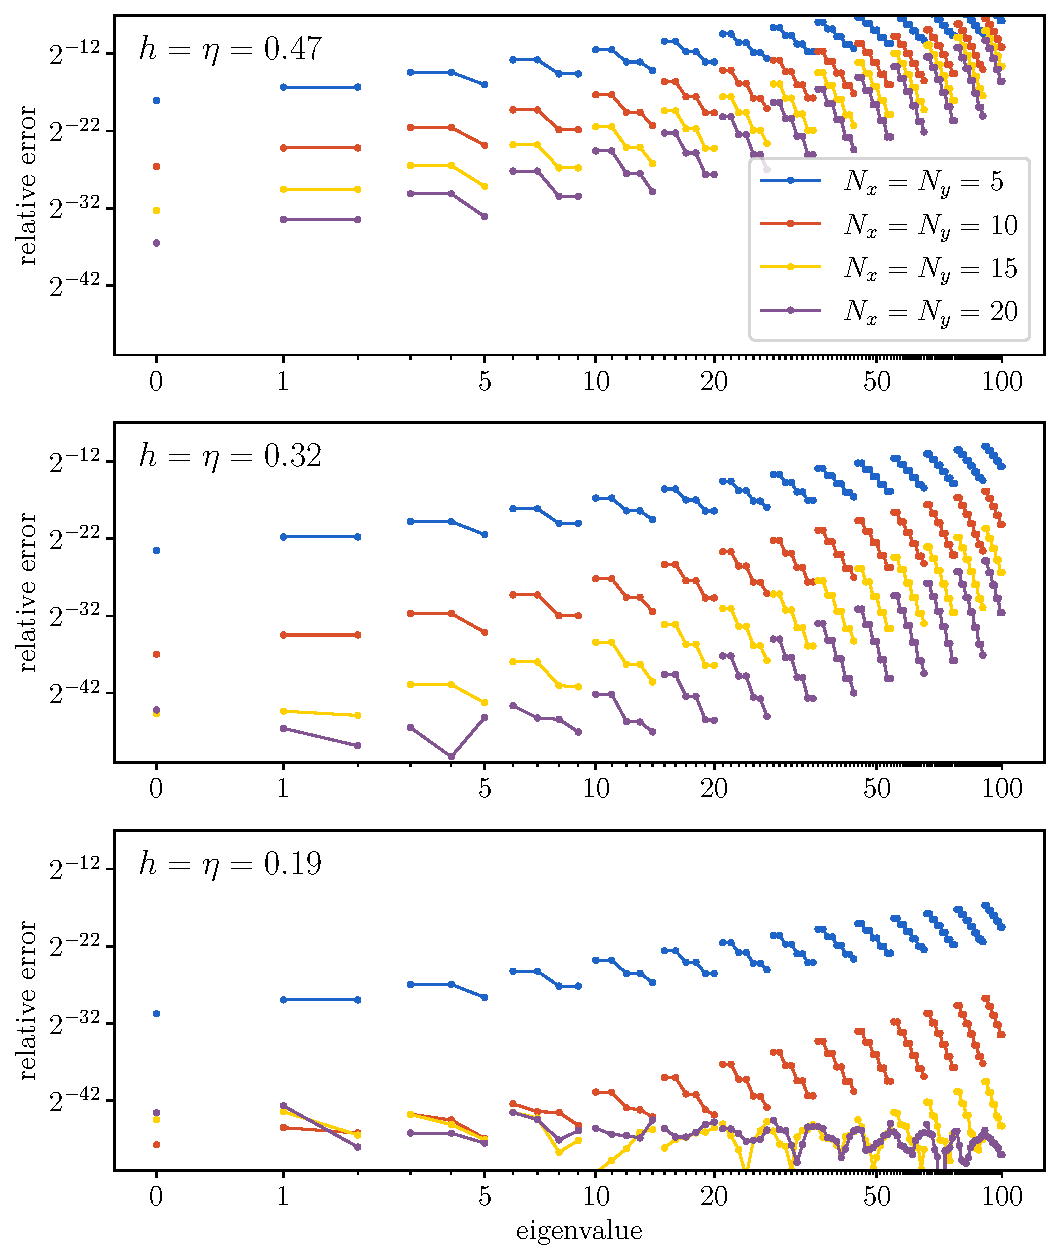
\includegraphics[width=\textwidth]{img/chapter4/fd_harmonic.pdf}
    \end{center}
    \caption{These graphs display the relative error of each of the first $100$ eigenvalues of the harmonic oscillator \eqref{equ:c4_fd_harmonic}, computed for different values of $h = \eta$ and $N_x = N_y$. Repeated eigenvalues are connected.}
    \label{fig:c4_fd_harmonic}
\end{figure}

As a first example we will replicate the results of \cite{wang_new_2009} for the harmonic oscillator:
\begin{equation}\label{equ:c4_fd_harmonic}
    -\nabla^2 \psi(x, y) + \left(x^2 + y^2\right) \psi(x, y) = E \psi(x, y)
\end{equation}
on the domain $[\numprint{-9.5}, \numprint{9.5}] \times [\numprint{-9.5}, \numprint{9.5}]$ with homogeneous Dirichlet boundary conditions. Notice that in \cite{wang_new_2009} the authors have chosen to scale the potential and eigenvalue by an extra factor of two. Here we did not do this, as such are computed eigenvalues will be twice as large. But, the relative errors remain the same.

In figure \ref{fig:c4_fd_harmonic} the relative errors for the first $100$ eigenvalues are plotted. This is done for $h = \eta \in \left\{\frac{19}{40}, \frac{19}{60}, \frac{19}{100}\right\}$ and $N_x = N_y \in \left\{ 5, 10, 20, 25 \right\}$. In these graphs a few things can be noted. Unsurprisingly, when $N_x = N_y$ is increased, the results become more accurate. And also, when $h = \eta$ is decreased, that is to say more grid points are used, the results also become more accurate. As is the case with most algorithms for approximating Schrödinger equations, when larger eigenvalues are computed, the accuracy decreases. The corresponding eigenfunctions become more and more oscillatory, and are thus more difficult to approximate accurately.

But most impressively, all these graphs were computed within a minute on a simple laptop. More detailed runtime analysis can be found in section \ref{sec:c4_nm_runtime}. Furthermore, the obtained results are also impressive. In the most accurate case $h= \eta = \frac{19}{100}$ and $N_x = N_y = 20$, the first $100$ eigenvalues are found with $45$ bits of precision, which is close to the ideal machine precision of $53$ bits.

To get a deeper understanding of this finite difference method it may be beneficial to study the asymptotic behavior of the error, with respect to the number of discretization points and the index of the eigenvalue. The finite difference approximation error can be used as a jumping point. Assume $N = N_x = N_y$, then the finite difference approximation of the second derivative of a function $f : \RR \to \RR$ is of the form:
$$
    f''(x) = \frac{1}{h^2}\sum_{i=-N}^{N} c_{i} f(x + i h) + \OO\mleft(h^{2N}\mright)\text{.}
$$

Going further with a theoretical analysis becomes unnecessarily difficult. We will estimate the order by using the numerical results for the first $100$ eigenvalues of the harmonic oscillator, calculated for the values of $h = \eta = \frac{1}{n}$ for $n \in \left\{20, 30, 40, 50, 60, 70, 80, 90, 100\right\}$. These $9$ different sets of parameters yield for each of the $100$ eigenvalues (with index $k \in \{1, 2, \dots, 100\}$) a data point. Next, through all these points we find the best fitting curve which follows the formula $\alpha_1 h^{\alpha_2} k^{\alpha_3}$. In this case we define the best fitting curve to be such that for the error $\epsilon_k^{(h)}$ (for each eigenvalue $k$ calculated with a step size of $h = \eta$), the following is minimized:
$$
    \sum_{k, h}\left|\log|\epsilon_{k}^{(h)}| - \log\mleft(c_1 h^{c_2} k^{c_3}\mright)\right|^2 \text{.}
$$

These best fits are summarized in the following table.
\begin{center}
    \begin{tabular}{r|cccc}
$N_x = N_y$ & $5$ & $10$ & $15$ & $20$ \\\hline\rule{0pt}{2.6ex}
Error & $\OO\mleft(h^{\numprint{3.90}}k^{\numprint{2.96}}\mright)$ & $\OO\mleft(h^{\numprint{5.78}}k^{\numprint{2.92}}\mright)$ & $\OO\mleft(h^{\numprint{6.61}}k^{\numprint{2.86}}\mright)$ & $\OO\mleft(h^{\numprint{7.07}}k^{\numprint{2.83}}\mright)$
\end{tabular}

\end{center}

It is important to note that these values are estimates, and are quite sensitive to the used values of $n$ and $k$. But, some trends are visible. We first note that increasing $N$ indeed increases the order in $h$ as well, maybe not as much as theoretical assumed $\OO\mleft(h^{2N}\mright)$, but nonetheless significantly. One of the reasons this theoretical value of $h^{2N}$ is not reached is because of the limited precision available in the \texttt{double} floating point type. For low eigenvalues, larger grids, and higher values of $N$, the error is so small that the numerical precision of the datatype becomes the main source of error. Another visible behavior is that a more accurate (higher order in $h$) method also has a larger exponent with respect to $k$. This means that higher eigenvalues are asymptotically less accurate. This property can also be seen in the graphs of figure \ref{fig:c4_fd_harmonic}, a virtual line through the points corresponding to $N = 5$ is less steep than a line through the points of $N = 10$.

For one-dimensional problems the behavior of the error with respect to $k$ has already been well studied and improved. In \cite{paine_correction_1981} expressions are constructed which provide a correction to the numeric approximation with a finite difference scheme for Sturm-Liouville problems. These correction formulae bring the order in $k$ down from $\OO(k^4h^2)$ to $\OO(k h^2)$. For multidimensional Schrödinger equations no such corrections are available, let alone for the extremely high order schemes considered here.

\paragraph{Zero potential} Besides the harmonic oscillator it is also instructive to consider the problem with a zero potential function on the domain $\Omega = [0, \pi] \times [0, \pi]$ and homogeneous Dirichlet boundary conditions. So, find all eigenvalues $E$ for which there exists an eigenfunction $\psi(x, y)$ on the domain with $\psi(x, y) = 0$ on $\dOmega$ such that the following holds:
\begin{equation}\label{equ:c4_fd_zero}
    -\nabla^2 \psi(x, y) = E \psi(x, y) \text{.}
\end{equation}

\begin{figure}
    \begin{center}
        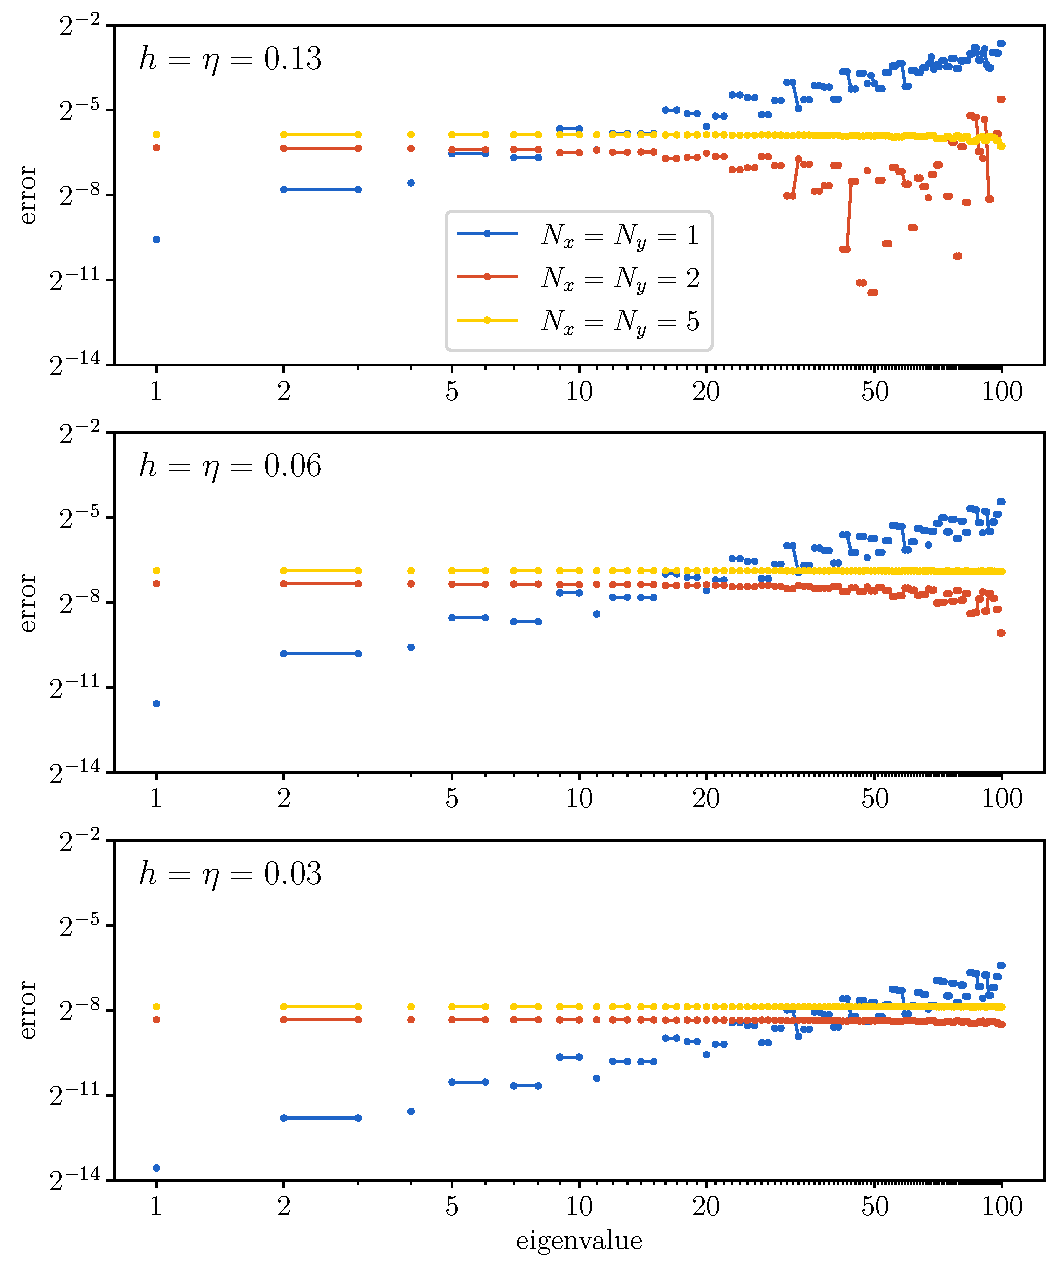
\includegraphics[width=\textwidth]{img/chapter4/fd_zero.pdf}
    \end{center}
    \caption{These graphs display the relative error of each of the first $100$ eigenvalues of a Schrödinger problem with a zero potential on the rectangular $[0, \pi] \times [0, \pi]$ domain with homogeneous Dirichlet boundary conditions \eqref{equ:c4_fd_zero}. This error is computed for different values of $h = \eta$ and $N_x = N_y$. Repeated eigenvalues are connected.}
    \label{fig:c4_fd_zero}
\end{figure}

By separation of variables, the exact solutions of this equation can be found: $\psi_{i, j}(x, y) = \sin(i x)\sin(j y)$ with eigenvalue $\lambda_{i,j} = i^2 + j^2$ for all $i, j \in \Nplus$. The first few of these eigenvalues are listed.
\begin{align*}
\lambda_{1,1} &= 2 & \lambda_{3,3} &= 18 & \lambda_{3,5} = \lambda_{5,3} &= 34\\
\lambda_{1,2} = \lambda_{2,1} &= 5 & \lambda_{2,4} = \lambda_{4,2} &= 20 & \lambda_{1,6} = \lambda_{6,1} &= 37\\
\lambda_{2,2} &= 8 & \lambda_{3,4} = \lambda_{4,3} &= 25 & \lambda_{2,6} = \lambda_{6,2} &= 40\\
\lambda_{1,3} = \lambda_{3,1} &= 10 & \lambda_{1,5} = \lambda_{5,1} &= 26 & \lambda_{4,5} = \lambda_{5,4} &= 41\\
\lambda_{2,3} = \lambda_{3,2} &= 13 & \lambda_{2,5} = \lambda_{5,2} &= 29 & \lambda_{3,6} = \lambda_{6,3} &= 45\\
\lambda_{1,4} = \lambda_{4,1} &= 17 & \lambda_{4,4} &= 32 & \lambda_{1,7} = \lambda_{5,5} = \lambda_{7,1} &= 50
\end{align*}%

In a certain way, these eigenvalues are more interesting than those from the harmonic oscillator, as their multiplicities are less predictable.

In figure \ref{fig:c4_fd_zero} the relative error in each of the first $100$ eigenvalues is displayed for different values of $h = \eta$ and $N_x = N_y$. When comparing this figure to the results of the harmonic oscillator \ref{fig:c4_fd_harmonic}, some striking differences can be seen. Maybe most surprisingly, increasing the order does not give more accurate results! For low eigenvalues the method with $N_x=N_y=1$ is most accurate, this is simply the second order central finite difference formula. When using higher order methods the error does not get any better than $2^{-8}\approx \numprint{0.00391}$, which is not at all as accurate as the results for the harmonic oscillator, where the error for $N_x=N_y = 5$ lies between $2^{-32} \approx \numprint{2.3e-10}$ and at most $2^{-16} \approx \numprint{1.5e-05}$. This is quite a disconcerting behavior for a numerical method to have.

These results bring to light one of the biggest drawbacks of the method from \cite{wang_new_2009}. This method only works if it is assumed that the eigenfunctions always are zero outside the domain. For the harmonic oscillator, this is the case, as $V(x, y) \to +\infty$ if $\|x, y\| \to +\infty$. For the zero potential function this is definitely not the case, the eigenfunctions are periodic. One could argue that, in theory, an eigenfunction may be anything outside the domain $\Omega$. So in particular, we could define them to be zero there. But, most numerical methods, and this method in particular, assume that solutions are sufficiently continuous. To cleanly define the problem, at least $C_0^2(\Omega)$ is needed, and when using $N^\text{th}$ order central finite difference schemes are used $C_0^{N}(\Omega)$ is implicitly assumed. And this assumption fails if we define the function to be zero outside $\Omega$.

To combat this issue, on the boundary of the domain asymmetric schemes could be used, the authors of \cite{wang_new_2009} did not do this. As an example, we have tabulated all relevant seven point formulae.
\begin{center}
    \begin{tabular}{ccc|c|ccccc|r}
$c_{-3}$ & $c_{-2}$ & $c_{-1}$ & $c_{0}$ & $c_{1}$ & $c_{2}$ & $c_{3}$ & $c_{4}$ & $c_{5}$ & error \\\hline
\rule{0pt}{3ex} $\frac{1}{90}$ & $- \frac{3}{20}$ & $\frac{3}{2}$ & $- \frac{49}{18}$ & $\frac{3}{2}$ & $- \frac{3}{20}$ & $\frac{1}{90}$ &  &  & $\OO\mleft(h^{6}\mright)$ \\
\rule{0pt}{3ex}  & $- \frac{13}{180}$ & $\frac{19}{15}$ & $- \frac{7}{3}$ & $\frac{10}{9}$ & $\frac{1}{12}$ & $- \frac{1}{15}$ & $\frac{1}{90}$ &  & $\OO\mleft(h^{5}\mright)$ \\
\rule{0pt}{3ex}  &  & $\frac{137}{180}$ & $- \frac{49}{60}$ & $- \frac{17}{12}$ & $\frac{47}{18}$ & $- \frac{19}{12}$ & $\frac{31}{60}$ & $- \frac{13}{180}$ & $\OO\mleft(h^{5}\mright)$ \\
\end{tabular}

\end{center}
There are two difficulties when using these formulae. Firstly, to reach the required order, one point more should be used. And secondly, when using asymmetric formulae the matrix from \eqref{equ:c4_fd_sparse_matrix} looses its symmetry as well. In principle this should not matter. But, in practice, many sparse matrix eigenvalue solvers are much more efficient when working with a real symmetric matrix.

    {\color{red}To do: give some results of this extension, maybe in a later subsection}

\paragraph{Hénon-Heiles} Lastly, ... {\color{red}To do}


\subsubsection{Computational cost of the method}

Finite differences are employed in many real-world applications, as they are easy to implement, yet are able to reach high accuracies. In practice, however, it is rare to see these very high orders used. In this setting these high orders seem to be very well applicable.

Yet, these finite difference methods are not without issues. One of the most prominent drawbacks is the expensive computations involved. To get accurate results, high orders combined with fine grids have to be used. This results in huge sparse matrices. And only thanks to their sparsity are algorithms able to compute the eigenvalues. Now, for higher order schemes, the matrices become less sparse, and as such more expensive to work with.

Alternatively, a method which is able to reduce the size of the matrices involved without losing accuracy may be preferable.

\subsection{A semi-discrete method}\label{sec:c4_semi_discrete}

{\color{red} To do: consider writing this intermediate method}

\section{Strands: A line-based collocation method}

In contrast to the previous methods, we propose a technique which is not necessarily restricted to cases where the domain is only a rectangle. So consider a finite domain $\Omega \subseteq \RR^2$ on which we are searching for eigenvalues $E \in \RR$ and eigenfunctions $\psi: \Omega \to \RR$ such that for a given potential $V : \Omega \to \RR$ the following holds
\begin{equation}\label{equ:c4_schrodinger_equation_new_method}
    -\nabla^2 \psi + V(x, y) \psi = E \psi\text{.}
\end{equation}
Still, we impose homogeneous Dirichlet boundary conditions: $\psi(x, y) = 0$ for $(x, y) \in \Omega$.

The main idea underlying this method is that we want to represent the eigenfunctions $\psi$ efficiently. A fully discretized method may represent eigenfunctions as its values on certain grid points. Our first attempt to develop a more continuous approximation of the eigenfunction used ideas from chapter \ref{cha:c3} and led to the creation of section \ref{sec:c4_semi_discrete}, where we have chosen to approximate the eigenfunction as a linear combination of well-chosen basis functions on parallel lines throughout the domain. This led to a continuous approximation along one direction and a discrete approximation along the other direction of the domain.

\begin{figure}
    \begin{center}
        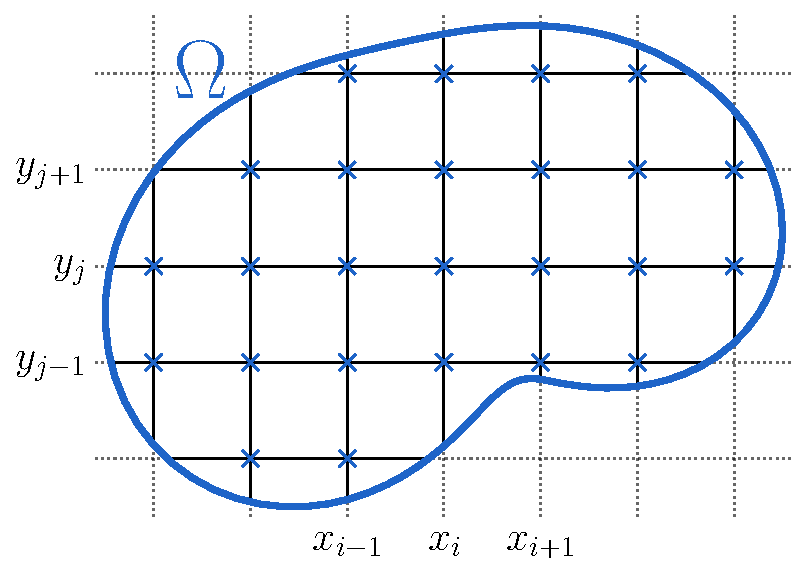
\includegraphics[width=.66\linewidth]{img/chapter4/the_method_grid.pdf}
        \caption{\label{fig:woven_method_grid} The grid}
    \end{center}
\end{figure}

We are now going to construct a new method in which we will bring this continuous approximation to both directions of the domain. For this, we place a grid over the domain $\Omega$, as can be seen in figure \ref{fig:woven_method_grid}. This grid does not need to be equidistant. When developing this new method we strived to allow for maximal flexibility, by avoiding as many restrictions on $\Omega$ as possible. This has as consequence that, because $\Omega$ does not have to be a rectangle, the number of intersections per grid line is not necessarily constant. Even worse, because we do not even require $\Omega$ to be convex, the intersection of a grid line with $\Omega$ may not be continuous. Upon formulating and implementing this new method, this varying number of intersections and these noncontinuous grid lines are some example of difficulties that arise by explicitly allowing more flexibility.

After placing the grid on $\Omega$, the next step is to approximate the unknown eigenfunction $\psi$ as a linear combination of basis functions on each of the grid lines. On the vertical line $x = x_i$, we denote these basis functions as $\beta_k^{(x_i)}(y)$, for each value of $k$. This yields the expression
\begin{equation}\label{equ:c4_expression_on_lines_x}
    \psi(x_i, y) = \sum_{k=0}^\infty c_k^{(x_i)} \beta_k^{(x_i)}(y) \text{.}
\end{equation}

For horizontal lines $y = y_j$, the basis functions $\beta_k^{(y_j)}(x)$ yield a similar expression
\begin{equation}\label{equ:c4_expression_on_lines_y}
    \psi(x, y_j) = \sum_{k=0}^\infty c_k^{(y_j)} \beta_k^{(y_j)}(x) \text{.}
\end{equation}

Notice that the domain of each of these $\beta$-fucntions is the intersection of its corresponding grid line with $\Omega$. As earlier stated, this domain may not be continuous. In theory this is not a problem, as long as the definition of $\beta$ allows this. And, it will. In practice when one wants to implement this, care has to be taken. It may be beneficial to construct multiple separate sets of basis functions for each of the continuous parts of the grid line. Because the theory has no problem with discontinuities, we will not burden the notation and explanation with this separation into continuous parts.

To ensure $\psi(x, y)$ is uniquely defined in each point in $\Omega$ we have to require that in each intersection point $(x_i, y_j)$, $\psi(x_i, y_j)$ has only one solution:
\begin{equation}\label{equ:c4_new_method_pre_matrix_equality}
    \psi(x_i, y_j) = \sum_{k=0}^\infty c_k^{(x_i)} \beta_k^{(x_i)}(y_j) = \sum_{k=0}^\infty c_k^{(y_j)} \beta_k^{(y_j)}(x_i)\text{.}
\end{equation}

Before deciding on which basis functions we should use, let us consider the Schrödinger equation \eqref{equ:c4_schrodinger_equation_new_method} on each intersection point $(x_i, y_j)$ with this new representation of $\psi$:
$$
    -\sum_{k=0}^\infty c_k^{(x_i)} \beta''^{(x_i)}_k(y_j) - \sum_{k=0}^\infty c_k^{(y_j)} \beta''^{(y_j)}_k(x_i) + (V(x_i, y_j) - E) \psi(x_i, y_j) = 0\text{.}
$$

This last formula suggest choosing $\beta_k^{(x_i)}$ and $\beta_k^{(y_j)}$, such that its second derivative contains, in a certain sense, $V(x_i, y_j)$. Together with the idea from chapter \ref{cha:c3} to use a one-dimensional Schrödinger equation, this leads us to propose $\beta_k^{(x_i)}$ to be the ordered eigenfunctions which satisfy the one dimensional Schrödinger equation
$$
    -\beta_k''^{(x_i)}(y) + \frac{V(x_i, y)}{2}\beta_k^{(x_i)}(y) = \lambda_k^{(x_i)} \beta_k^{(x_i)}(y)
$$
with homogeneous Dirichlet boundary conditions. The domain for this one-dimensional problem is the intersection of the vertical line $x = x_i$ and the two-dimensional domain $\Omega$. Similarly, for the horizontal line $y = y_j$, we propose $\beta_k^{(y_j)}(x)$ to be the eigenfunctions of
$$
    -\beta_k''^{(y_j)}(x) + \frac{V(x, y_j)}{2}\beta_k^{(y_j)}(x) = \lambda_k^{(y_j)} \beta_k^{(y_j)}(x)
$$
with homogeneous Dirichlet boundary conditions, and as domain the intersection of $y = y_j$ and $\Omega$.

By choosing half the original potential in each of the approximations, in each intersection $(x_i, y_j)$, equation \eqref{equ:c4_schrodinger_equation_new_method} simplifies, and $V(x, y)$ disappears:
\begin{equation}\label{equ:c4_new_method_pre_matrix}
    \sum_{k=0}^\infty \lambda_k^{(x_i)} c_k^{(x_i)} \beta^{(x_i)}_k(y_j) + \sum_{k=0}^\infty \lambda_k^{(y_j)} c_k^{(y_j)} \beta_k^{(y_j)}(x_i) = E \psi(x_i, y_j) \text{.}
\end{equation}

Notice that in this expression only $E$ (the eigenvalue) and $c_k^{(x_i)}$ and $c_k^{(y_j)}$ are unknown, as $\psi(x_i, y_j)$ depends linearly on $c_k^{(x_i)}$ and $c_k^{(y_j)}$. So, expression \eqref{equ:c4_new_method_pre_matrix} is, in fact, a linear problem.

Before writing this as a matrix-problem, we first have to limit the extent of the sum. It is, of course, impossible to implement these formulas while the function bases are still infinite. Therefor, we limit the basis on the line $x = x_i$ to the first $K_{x_i}$ functions and to the first $K_{y_j}$ functions on the line $y = y_j$. Notice that the size of a basis on each line, should not be greater than the number of intersections on that line. If the basis size is too large, the system \eqref{equ:c4_new_method_pre_matrix_equality} would be underdetermined. In this case, solutions will no longer be uniquely defined, which is a problem. In contrast, if the basis size is smaller, the system \eqref{equ:c4_new_method_pre_matrix_equality} would be overdetermined. This does not lead to issues, because we can reformulate it as finding solutions in a least squares sense.

With these finite sums equations \eqref{equ:c4_new_method_pre_matrix_equality} and \eqref{equ:c4_new_method_pre_matrix} become, on the intersection $(x_i, y_j)$:
\begin{align}
     & \sum_{k=0}^{K_{x_i}-1} \lambda_k^{(x_i)} c_k^{(x_i)} \beta^{(x_i)}_k(y_j) + \sum_{k=0}^{K_{y_j}-1} \lambda_k^{(y_j)} c_k^{(y_j)} \beta_k^{(y_j)}(x_i)\nonumber                                  \\
     & \qquad\qquad\qquad     = \sum_{k=0}^{K_{x_i}-1} c_k^{(x_i)} \beta_k^{(x_i)}(y_j) = \sum_{k=0}^{K_{y_j}-1} c_k^{(y_j)} \beta_k^{(y_j)}(x_i) \text{.}\label{equ:c4_new_method_pre_matrix_unified}
\end{align}
The introduction of appropriate vectors and matrices will allow us to translate \eqref{equ:c4_new_method_pre_matrix_unified} into a matrix problem. The unknowns will be summarized into the two vectors $\vb{c_x}$ and $\vb{c_y}$, with sizes $n_x := \sum_i K_{x_i}$ and $n_y := \sum_j K_{y_j}$ respectively:
\begin{align*}
    \vb{c_x}            & = \transpose{\begin{pmatrix} c_0^{(x_0)} & c_1^{(x_0)} & \dots & c_{K_{x_0}-1}^{(x_0)} & c_0^{(x_1)} & c_1^{(x_1)} & \dots \end{pmatrix}}         \\
    \text{and }\vb{c_y} & = \transpose{\begin{pmatrix} c_0^{(y_0)} & c_1^{(y_0)} & \dots & c_{K_{y_0}-1}^{(y_0)} & c_0^{(y_1)} & c_1^{(y_1)} & \dots \end{pmatrix}}\text{.}
\end{align*}

Furthermore, we introduce the $n_x \times n_x$ diagonal matrix $\vb{\Lambda_x}$ and the $n_y \times n_y$ diagonal matrix $\vb{\Lambda_y}$ which contain the eigenvalues of the one-dimensional Schrödinger problems used to define the basis functions:
\begin{align*}
    \vb{\Lambda_x}            & = \diag\begin{pmatrix} \lambda_0^{(x_0)} & \lambda_1^{(x_0)} & \dots & \lambda_{K_{x_0}-1}^{(x_0)} & \lambda_0^{(x_1)} & \lambda_1^{(x_1)} & \dots \end{pmatrix}         \\
    \text{and }\vb{\Lambda_y} & = \diag\begin{pmatrix} \lambda_0^{(y_0)} & \lambda_1^{(y_0)} & \dots & \lambda_{K_{y_0}-1}^{(y_0)} & \lambda_0^{(y_1)} & \lambda_1^{(y_1)} & \dots \end{pmatrix}\text{.} \\
\end{align*}

\begin{figure}
    \begin{center}
        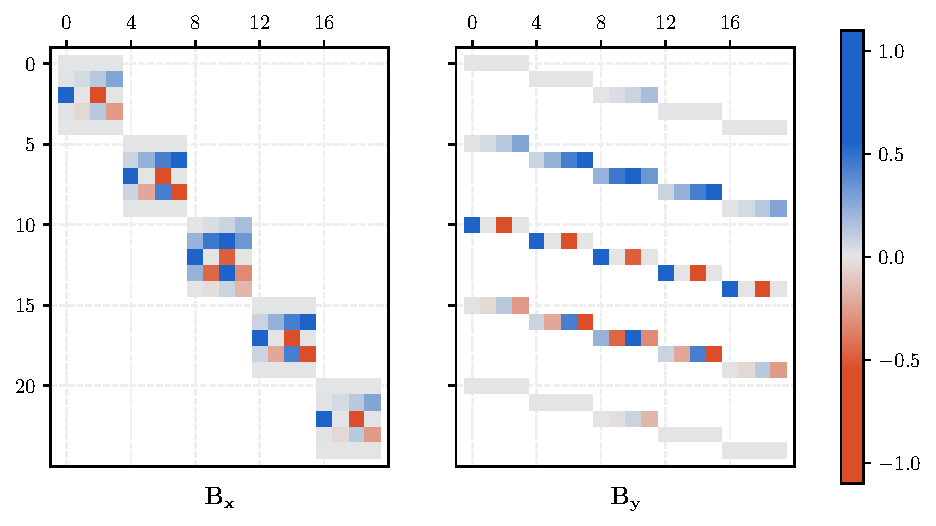
\includegraphics[width=\textwidth]{img/chapter4/new_method_beta.pdf}
        \caption{The non-zero entries of the matrices $\vb{B_x}$ and $\vb{B_y}$ from equation \eqref{equ:c4_new_method_beta_definition} are visualized. These were calculated on the problem from section \ref{sec:c4_numerical_ixaru} with a 5 by 5 internal grid and $K_{x_i} = K_{y_j} = 4$ basis functions per line. In practice, these matrices are much larger.}
        \label{fig:c4_new_method_beta}
    \end{center}
\end{figure}

Lastly we define the matrices which contain the values of the basis functions in each of the grid points. For this let us define $m$ as the total number of intersection points. Now, we define the $m \times n_x$ matrix $\vb{B_x}$ and the $m \times n_y$ matrix $\vb{B_y}$. Each row $r_{i,j}$ of these matrices correspond to a grid point $(x_i, y_j)$. The non-zero entries on each of the rows $r_{i,j}$ of the matrices $\vb{B_x}$ and $\vb{B_y}$ can be calculated as
\begin{align}
    \left(\vb{B_x}\right)_{r_{i,j}, o^{(x)}_{i} + k} & =  \beta_{k}^{(x_i)}(y_j) \text{ for $k \in \{0, 1, \dots, K_{x_i} - 1\}$ }   \nonumber                               \\
    \text{and }
    \left(\vb{B_y}\right)_{r_{i,j}, o^{(y)}_{j} + k} & =  \beta_{k}^{(y_j)}(x_i) \text{ for $k \in \{0, 1, \dots, K_{y_i} - 1\}$.} \label{equ:c4_new_method_beta_definition}
\end{align}
In this expression the values $o^{(x)}_{i}$ and $o^{(y)}_{j}$ are certain offsets depending on the row. These offsets are defined as: $o^{(x)}_{i} := \sum_{i' < i} K_{x_{i'}}$ and $o^{(y)}_{j} := \sum_{j' < j} K_{y_{j'}}$. To aid an intuitive understanding of the $\vb{B_x}$ and $\vb{B_y}$ matrices, figure \ref{fig:c4_new_method_beta} provides a schematic view of them, calculated from a small numerical example.

As promised, these definitions allow us to rewrite the system \eqref{equ:c4_new_method_pre_matrix_unified} with $m$ equations more compactly as:
\begin{equation}\label{equ:c4_nm_matrix_compact}
    \vb{B_x} \vb{\Lambda_x}\vb{c_x} + \vb{B_y} \vb{\Lambda_y}\vb{c_y} = E \vb{B_x} \vb{c_x} = E \vb{B_y} \vb{c_y}\text{.}
\end{equation}

This formulation is not yet reminiscent of any classical linear algebra problem. One of the unfamiliar parts of this expression is the fact that there are two vectors of unknowns, another unfamiliar part is that \eqref{equ:c4_nm_matrix_compact} defines, in fact, two different equations.
\begin{equation}
    \begin{cases}
        \vb{B_x} \vb{\Lambda_x}\vb{c_x} + \vb{B_y} \vb{\Lambda_y}\vb{c_y} = E \vb{B_x} \vb{c_x} \\
        \vb{B_x} \vb{c_x} = \vb{B_y} \vb{c_y}
    \end{cases} \label{equ:c4_new_method_first_matrix_problem}
\end{equation}

There are a few strategies to further translate this problem into a form for which efficiently implemented and well-studied algorithms exist. Ideally, the solution would take the sparsity of the involved matrices into account.

\subsection{Solving the matrix approximation}

As a first strategy we investigated how this problem can be directly transformed into a standard mathematical problem.

\subsubsection{Direct transformation into an eigenvalue problem}

We tackle equation \eqref{equ:c4_new_method_first_matrix_problem} by rewriting it as
$$
    \begin{cases}
        \vb{B_x} \vb{\Lambda_x}\vb{c_x} + \vb{B_y} \vb{\Lambda_y}\vb{c_y} = E \vb{B_x} \vb{c_x} \\
        \vb{B_x} \vb{\Lambda_x}\vb{c_x} + \vb{B_y} \vb{\Lambda_y}\vb{c_y} = E \vb{B_y} \vb{c_y} \\
    \end{cases}\text{.}
$$
This system can be seen as the following generalized rectangular eigenvalue problem:
\begin{equation}\label{equ:c4_new_method_alternative_system}
    \begin{pmatrix}
        \vb{B_x} \vb{\Lambda_x} & \vb{B_y} \vb{\Lambda_y} \\
        \vb{B_x} \vb{\Lambda_x} & \vb{B_y} \vb{\Lambda_y}
    \end{pmatrix} \begin{pmatrix}
        \vb{c_x} \\ \vb{c_y}
    \end{pmatrix} = E \begin{pmatrix}
        \vb{B_x} & \vb{0} \\ \vb{0} & \vb{B_y}
    \end{pmatrix} \begin{pmatrix}
        \vb{c_x} \\ \vb{c_y}
    \end{pmatrix}\text{.}
\end{equation}

At first glance this may seem to enable us to solve the problem elegantly. But, there are a few issues apparent with this translation. One of the most visible problems is that we have translated this into a matrix problem which is twice as large as the original matrices $\vb{B_x}$ and $\vb{B_y}$ in both rows and columns. On the other hand, one can argue that the matrices are clearly sparse. The matrices $\vb{B_x}$ and $\vb{B_y}$ are sparse indeed, but the problem is that there are few algorithms available that are even able to solve a generalized rectangular eigenvalue problem, let alone a sparse one.

But a lack of sparse implementations does not deter us from trying out some numerical experiments. In this first experiment we will have to fall back to algorithms working on dense matrices. Of course, the runtime will suffer, but from a numerical point of view the results will still be valuable.

Consider the Schrödinger equation with the harmonic oscillator potential:
$$
    -\nabla^2\psi(x, y) + \left(x^2 + y^2\right) \psi(x, y) = E \psi(x, y)
$$
on the domain $[-9.5, 9.5] \times [-9.5, 9.5]$ with homogeneous Dirichlet boundary conditions\footnote{We also considered this problem in section \ref{sec:c4_fd_numerical}.}. We apply the described method on a grid with 30 lines in each direction and 16 basis functions per line. This yields $900\times 480$ matrices $\vb{B_x}$ and $\vb{B_y}$, and the rectangular problem from \eqref{equ:c4_new_method_alternative_system} has \numprint{1800} equations and \numprint{960} variables. As this eigenvalue problem is heavily overdetermined, we have to considered that solutions will only be accurate in a least squares sense. Much research is already dedicated to solving this kind of problem, as such we will, for now, use the first method from \cite{hua_svd_1991} to find solutions. Later on, we will explore the world of generalized rectangular eigenvalue problems.

If we write equation \eqref{equ:c4_new_method_alternative_system} symbolically as $\vb{A} \vb{c} = E \vb{D} \vb{c}$, and the truncated singular value decomposition of $\vb{D}$ as $\vb{D} = \vb{U_D} \vb{\Sigma_D} \vb{V_D^\adjointsign}$, then any solution of \eqref{equ:c4_new_method_alternative_system} will also be a solution of the generalized square eigenvalue problem
$$
    \vb{U_D^\adjointsign} \vb{A} \vb{V_D} \vb{v} = E \vb{\Sigma_D} \vb{v} \text{,}
$$
with $\vb{c} = \vb{V_D} \vb{v}$. Applying this method to the numerical problem yields 840 eigenvalues. Firstly, it is important to remark that the resulting values are elements of $\CC$. But, in this case, the imaginary part of all values lies between \numprint{-1.68e-14} and \numprint{1.68e-14}, so all values may be considered real. The lowest few values are given:
$$
    \underbrace{
        \numprint{-2.85e-14} \quad \dots \quad \numprint{5.39e-14}
    }_\text{256 values close to zero} \quad \numprint{2.00} \quad \numprint{3.93} \quad \numprint{3.93} \quad \numprint{4.00} \quad \numprint{4.00} \quad \dots
$$

This can be more compactly summarized when the number of times an eigenvalue is (up to a precision of $10^{-6}$) repeated is indicated by a subscript:

\begin{tabular}{ccccccccccc}
    $\numprint{0.00}_{256}$ & $\numprint{2.00}$ & $\numprint{3.93}_2$ & $\numprint{4.00}_2$ & $\numprint{5.36}_2$ & $\numprint{6.00}_3$ & $\numprint{6.78}_2$ & $\numprint{6.87}_2$ & $\numprint{8.00}_4$ & $\dots$
\end{tabular}

One immediately notices the many returned zero values. Some of these can be explained by the structure of the matrix on the left-hand size of \eqref{equ:c4_new_method_alternative_system}. This is a $2\cdot 900 \times (480 + 480)$ matrix with repeated rows. The rank is thus at most $900$, which explains $960 - 900 = 60$ zero eigenvalues. The others are more difficult to explain, but suggestions can be found in the fact that $\vb{B_x} \vb{\Lambda_x} \vb{c_x}$ and $\vb{B_y} \vb{\Lambda_y} \vb{c_y}$ describe (up to a least squares approximation) the same points. So, $\vb{c_x}$ and $\vb{c_y}$ are not independent, which implies that the rank of the matrix $\begin{pmatrix} \vb{B_x} \vb{\Lambda_x} & \vb{B_y} \vb{\Lambda_y}\end{pmatrix}$ will probably not be maximal. But, these zero eigenvalues indicate another problem. Namely, that for these values it is not at all guaranteed that $\vb{B_x} \vb{c_x} = \vb{B_y} \vb{c_y}$. So, these eigenvalues will be nonsensical in the context of the original Schrödinger problem.

Remember that the true eigenvalues of the harmonic oscillator are 2, 4, 4, 6, 6, 6, 8, 8, 8, 8, \dots. And, we notice that these true values can indeed be found in our solutions, but also many other values are present. Because the method from \cite{hua_svd_1991} for solving generalized rectangular eigenvalue problems may return more solutions than the original problems has, we still have to filter some out. One way to only end up with true eigenvalues is by substituting them back into the original problem \eqref{equ:c4_new_method_first_matrix_problem} and verifying the residuals of both equations:
$$
    r_1 = \left\| \vb{B_x} \vb{\Lambda_x} \vb{c_x} + \vb{B_y} \vb{\Lambda_y} \vb{c_y} - \frac{E}{2}\left(\vb{B_x}\vb{c_x} + \vb{B_y}\vb{c_y}\right) \right\| \text{ and } r_2=\left\| \vb{B_x} \vb{c_x} - \vb{B_y} \vb{c_y} \right\|\text{.}
$$

The found possible eigenvalue with the lowest residuals $r_1$ and $r_2$ are also true eigenvalues of the Schrödinger problem. When we sort all possibilities by their first residual $r_1$ we obtain the following table.

\begin{center}
    \begin{tabular}{r|rrrrr}
$E$ & \numprint{2.000000} & \numprint{4.000000} & \numprint{4.000000} & \numprint{6.000000} & \numprint{7.999998} \\\hline
$r_1$ & \numprint{1.5e-5} & \numprint{4.7e-4} & \numprint{4.7e-4} & \numprint{4.9e-4} & \numprint{5.0e-3} \\
$r_2$ & \numprint{1.2e-5} & \numprint{2.3e-4} & \numprint{2.3e-4} & \numprint{1.6e-4} & \numprint{1.2e-3}
\end{tabular}

\begin{tabular}{r|rrrrr}
$E$ & \numprint{7.999998} & \numprint{9.999997} & \numprint{9.999997} & \numprint{10.000006} & \numprint{8.000007} \\\hline
$r_1$ & \numprint{5.0e-3} & \numprint{6.6e-3} & \numprint{6.7e-3} & \numprint{1.0e-2} & \numprint{1.4e-2} \\
$r_2$ & \numprint{1.2e-3} & \numprint{1.3e-3} & \numprint{1.3e-3} & \numprint{2.1e-3} & \numprint{3.5e-3}
\end{tabular}

\begin{tabular}{r|rrrrr}
$E$ & \numprint{8.000007} & \numprint{13.999988} & \numprint{5.999974} & \numprint{5.999974} & \numprint{10.000151} \\\hline
$r_1$ & \numprint{1.4e-2} & \numprint{1.9e-2} & \numprint{3.8e-2} & \numprint{3.8e-2} & \numprint{4.8e-2} \\
$r_2$ & \numprint{3.5e-3} & \numprint{2.7e-3} & \numprint{1.3e-2} & \numprint{1.3e-2} & \numprint{9.6e-3}
\end{tabular}


\end{center}

Here, we see that when the first residual $r_1$ is low, the other is as well. Also, in the first few eigenvalues, only true solutions are present.

Upon studying this direct method to solve the system of equations \eqref{equ:c4_new_method_first_matrix_problem}, we have noticed some drawbacks. Firstly, the proposed system \eqref{equ:c4_new_method_alternative_system} is, in a certain sense, twice as large as the discrete problem we started from. Eigenvalue algorithms are at least cubic in complexity. So, this doubling in size implies an eightfold runtime penalty. Secondly, and numerically interesting, we obtain many more `solutions' than the ones we are looking for. Each generalized eigenvalue, with its eigenvector, has to be computed and checked against the residuals. Many eigenvalues will be thrown away.

\subsubsection{Restriction to a null space}\label{sec:nm_by_restriction}

One improvement we can make to the runtime is by not solving a system that is twice as large, but by solving two smaller systems. Furthermore, instead of ending up with too many eigenvalues and trying to filter out the wrong ones, we have devised a way to, a priori, limit the number of solutions. The idea here is that, before solving an eigenvalue problem, we solve the second equation of \eqref{equ:c4_new_method_first_matrix_problem} and only take those solutions into account.

The first equation resembles a generalized rectangular eigenvalue problem, the second is a classical linear system. Let us only consider $n_x + n_y$ dimensional vectors $\vb{c} = \transpose{\begin{pmatrix}\transpose{\vb{c_x}} & \transpose{\vb{c_y}} \end{pmatrix}}$ which solve
$$
    \begin{pmatrix}\vb{B_x} & -\vb{B_y} \end{pmatrix} \vb{c} = \vb{0}\text{.}
$$
This allows us to unify $\vb{c_x}$ and $\vb{c_y}$, while ensuring $\vb{B_x} \vb{c_x} = \vb{B_y} \vb{c_y}$ is satisfied. To expand on this idea, we will write $\vb{c}$ to be an element of the right kernel of  $\begin{pmatrix}\vb{B_x} & -\vb{B_y} \end{pmatrix}$. For this define the columns of the $(n_x + n_y) \times z$ matrix $\vb{Z}$ to be a basis of this right kernel:
\begin{equation}\label{equ:c4_null_space_kernel}
    \begin{pmatrix}\vb{B_x} & -\vb{B_y} \end{pmatrix} \vb{Z} = \vb{0}\text{.}
\end{equation}

Computing this kernel numerically is definitely not trivial. For rectangular matrices, there are a few well-known methods to compute the kernel. In the next paragraphs we will explore these methods and consider how well they are suited for our problem. For ease of notation we will be solving the rectangular system $\vb{A} \vb{Z} = \vb{0}$ with $\vb{A}$ a (sparse) $m\times n$ matrix and $\vb{Z}$ a yet unknown $n \times z$ matrix, whose columns are a basis for the right null space of $\vb{A}$.

One of the first methods for finding the nullspace of a matrix one finds browsing the literature is by computing its singular value decomposition. For the extended background about the singular value decomposition we refer to \cite[section~2.4]{golub_matrix_2013}. In this book the following theorem can be found.

\begin{theorem}
    Let $\vb{A} \in \RR^{m \times n}$ be a real $m \times n$ matrix with singular value decomposition\footnote{In this expression the matrix $\vb{U}$ ($\vb{V}$ respectively) are orthogonal $m \times m$ ($n \times n$ respectively) matrices. $\vb{\Sigma}$ is a diagonal $m \times n$ matrix with the ordered singular values on the diagonal: $\sigma_1 \geq \sigma_2 \geq \dots \geq \sigma_{\min(m, n)}$. }
    $$
        \vb{A} = \vb{U}\vb{\Sigma}\transpose{\vb{V}}\text{,}
    $$
    and ordered singular values $\sigma_1 \geq \sigma_2 \geq \dots \geq \sigma_p$ with $p = \min(m, n)$.
    If $\vb{A}$ has $r$ positive singular values, then\footnote{The nullspace $\opnull(\vb{A})$ of $\vb{A}$ is the vector space with all vectors $\vb{x}$ for which $\vb{A} \vb{x} = \vb{0}$. The range $\opran(\vb{A})$ is the vector space with all vectors $\vb{y}$ such that there exists a vector $\vb{x}$ such that $\vb{A}\vb{x} = \vb{y}$} $\oprank(A) = r$ and
    \begin{align*}
        \opnull(\vb{A}) & = \opspan\{\vb{v}_{r+1}, \dots, \vb{v}_{n}\}\text{,} \\
        \opran(\vb{A})  & = \opspan\{\vb{u}_{1}, \dots, \vb{u}_{r}\}\text{,}
    \end{align*}
    with $\vb{u}_i$ the $i^\text{th}$ column of $\vb{U}$, analogous $\vb{v}_i$ the $i^\text{th}$ column of $\vb{V}$.
\end{theorem}

The singular value decomposition gives us a constructive way to find a basis of the null space of a matrix $\vb{A}$. For dense matrices this works very well, but is computationally quite expensive. For sparse matrices the story is more complicated. There are many available routines for calculating singular value decomposition, some of them are constructed specifically for computing the singular value decomposition, others are adapted from symmetric eigenvalue solvers on the matrix $\transpose{\vb{A}}\vb{A}$ or on $\vb{A}\transpose{\vb{A}}$, whichever is more efficient, for example: \slepc \cite{hernandez_slepc_2005}, \spectra \cite{qiu_yixuan_2022} or \scipy \cite{virtanen_scipy_2020} with \arpack \cite{lehoucq_arpack_1998}. We have experimented with many solvers. One of the first difficulties is that all of them require specifying beforehand how many singular values are required. But, in our case, the dimension of the null space is unknown, so it is impossible to say exactly. The solver which seemed most promising to combat this issue was \slepc \cite{hernandez_slepc_2005}. There one is able to provide a custom condition until which the solver will continue to find singular values. In our case, we could provide that as long as the singular values are close to zero, the search should continue. But, on the other hand, the algorithms used there are using a small-dimensional subspace in which convergence to the eigenvectors happens. This space should at least have as many dimensions as the number of eigenvalues required, and has to be specified beforehand. As noted previously, in our case, this is difficult. But, even ignoring this complication, and just specifying a sufficiently high number of required singular values, did not solve it either. All algorithms had trouble to reliably converge to the required number of singular values. In the simplest test problem, the best result we were able to obtain this way were a few dozen of the smallest singular values, where a few hundred were required.

Another popular\cite{trefethen_numerical_1997} method to find the nullspace of a matrix is by using a QR-decomposition with pivoting. For this we decompose the $m \times n$ matrix $\vb{A}$ as $\transpose{\vb{A}}\vb{E} = \vb{Q} \vb{R}$, with $\vb{E}$ a $m\times m$ permutation matrix, $\vb{Q}$ a square $n \times n$ orthogonal matrix and $\vb{R}$ a $n \times m$ rectangular upper triangular matrix, with the elements on its diagonal sorted (descending in absolute value). To find the kernel we now consider for which vectors $\vb{z}$ the expression $\vb{A} \vb{z} = \vb{E}\transpose{\vb{R}}\transpose{\vb{Q}}\vb{z}$ becomes zero. Notice that this only happens when $\vb{z}$ is in the linear span of the columns of $\vb{Q}$ corresponding to a diagonal item in $\vb{R}$ that is (close to) zero and, if $n > m$ the last $n - m$ columns of $\vb{Q}$. So an orthogonal basis of the null space of $\vb{A}$ can be found in a selection of columns of $\vb{Q}$ in the QR-decomposition of $\transpose{\vb{A}}$. For dense matrices this procedure also works very well. We can quite easily compute the full kernel with built-in QR routines. Upon selecting which columns to include, the diagonal elements of $\vb{R}$ can even be used to take into account a prespecified tolerance. It is also valuable to notice that computing a QR decomposition is significantly more efficient than finding all singular values. So, for dense matrices, this second method is preferred. But for sparse matrices, the story is, again, quite different. There are many well-tested routines to compute a sparse QR decomposition, for example SuiteSparseQR \cite{davis_algorithm_2011} and \Eigen's QR \cite{guennebaud_eigen_2010}. Yet, we have tested this algorithm with both solvers, without success. \Eigen does not contain a rank revealing QR decomposition, and as such is unable to compute the full kernel. SuiteSparseQR on the other hand was sometimes able to compute the kernel, but this computation was each time very sensitive to the tolerances for when pivoting should happen and which columns of $\vb{Q}$ to include. Even worse, the perfect `tolerance' was different for each test problem, or even for the same problem with different parameters.

In conclusion, coming back to equation \eqref{equ:c4_null_space_kernel}, for now we will ignore the sparsity present and use the algorithm for the dense QR-decomposition present in \Eigen \cite{guennebaud_eigen_2010}.

The vector $\vb{c}$ can now be written as a linear combination of columns of $\vb{Z}$:
$$
    \vb{c} = \begin{pmatrix}\vb{c_x} \\ \vb{c_y} \end{pmatrix} = \begin{pmatrix} \vb{Z_x} \\ \vb{Z_y} \end{pmatrix}  \vb{u} = \vb{Z} \vb{u} \text{.}
$$
Another benefit of considering $\vb{Z}\vb{u}$, besides only considering solutions of $\vb{B_x} \vb{c_x} = \vb{B_y} \vb{c_y}$, is that we unified the two vectors of unknowns $\vb{c_x}$ and $\vb{c_y}$ into one (much) smaller vector $\vb{u}$. This simplifies the two problems of equation \eqref{equ:c4_new_method_first_matrix_problem} into
$$
    \begin{pmatrix}
        \vb{B_x}\vb{\Lambda_x} & \vb{B_y}\vb{\Lambda_x}
    \end{pmatrix} \vb{Z} \vb{u} = E \vb{B_x} \vb{Z_x} \vb{u} = E \vb{B_y} \vb{Z_y} \vb{u} \text{.}
$$
For the right-hand side, by construction $\vb{B_x} \vb{Z_x} = \vb{B_y} \vb{Z_y}$. Now, this problem has become a generalized rectangular eigenvalue problem.

    {\color{red}To do: Finding solutions of generalized rectangular eigenvalue problems}

\subsubsection{Least squares approximation}

For dense matrices, the previous technique works very well. The correct eigenvalues are found within very reasonable computation time. But, if extremely high accuracies are required, the used grid size should be increased. This also has a significant impact on the size of the involved matrices. As these become larger, using their sparsity becomes a necessity. This is where both of the previous techniques to solve \eqref{equ:c4_new_method_first_matrix_problem} fall short. There, existing algorithms for sparse matrices were not able to do the required computations efficiently and accurately. To combat this, we have developed an alternative method. Explicitly tuned to be able to use the sparsity of the matrices.

We start with the observation that classical matrix problems normally do not contain two vectors of unknowns. So, we need a way to unify them. With the previous technique we considered vectors in the right kernel of a given matrix. We have discovered that this is surprisingly difficult to compute, while respecting the sparsity of the matrices involved. As an alternative to unify $\vb{c_x}$ and $\vb{c_y}$, one could fix $\vb{c_x}$ and compute $\vb{c_y}$ as the least-squares solution of $\vb{B_x}\vb{c_x} = \vb{B_y}\vb{c_y}$. Or, the other way around, fix $\vb{c_y}$ and computed $\vb{c_x}$. Both seem like artificial asymmetric choices. Therefor, we propose to find an $m$-dimensional vector $z$, such that $\vb{c_x}$ and $\vb{c_y}$ can be calculated as least square solutions of $\vb{B_x}\vb{c_x} = \vb{B_y}\vb{c_y} = \vb{z}$. With normal equations, we can define this more formally as
\begin{align*}
    \vb{c_x}            & = \left(\vb{B_x^\transposesign} \vb{B_x}\right)^{-1} \vb{B_x^\transposesign} \vb{z}          \\
    \text{and }\vb{c_y} & = \left(\vb{B_y^\transposesign} \vb{B_y}\right)^{-1} \vb{B_y^\transposesign} \vb{z} \text{.}
\end{align*}

Notice that the computation of $\left(\vb{B_x^\transposesign} \vb{B_x}\right)^{-1}$ is not at all as difficult as this may seem: $\vb{B_x}$ is a block diagonal matrix. So, these computations, calculating an inverse or multiplying with another block diagonal matrix, can be done for each of the much smaller dense subblocks on the diagonal. From figure \ref{fig:c4_new_method_beta} we know that the matrix $\vb{B_y}$ is not block diagonal. But, if we apply an appropriate $m \times m$ permutation matrix $\vb{P}$ we can obtain that $\vb{\widetilde{B}_y} := \vb{P} \vb{B_y}$ is, in fact, also a block diagonal matrix. So, the computation of $\vb{c_y}$ can be written as:
$$
    \vb{c_y} = \left(\vb{\widetilde{B}_y^\transposesign} \vb{\widetilde{B}_y}\right)^{-1} \vb{\widetilde{B}^\transposesign_y} \vb{P} \vb{z} \text{.}
$$
And again, as the involved matrices (except $\vb{P}$) are block diagonal, all computation can be delegated to the much smaller dense subblocks of $\vb{\widetilde{B}_y}$.

Numerically, directly computing inverse matrices should be avoided. Therefor, we compute the matrix $\vb{Z_x} := \left(\vb{B_x^\transposesign} \vb{B_x}\right)^{-1} \vb{B_x^\transposesign}$ as the least squares solution of $\vb{B_x} \vb{Z_x} = \vb{I}_{m \times m}$, and analogous for $\vb{Z_y} = (\vb{\widetilde{B}_y^\transposesign} \vb{\widetilde{B}_y})^{-1} \vb{\widetilde{B}^\transposesign_y}$. And again, all these computations can be executed on each of much smaller dense diagonal blocks.

The expressions for $\vb{c_x}$ and $\vb{c_y}$ now allow us to rewrite the first equation of \eqref{equ:c4_new_method_first_matrix_problem} into
\begin{equation}\label{equ:c4_nm_sparse_system}
    \left(\vb{B_x}\vb{\Lambda_x} \vb{Z_x} + \transpose{\vb{P}}\vb{\widetilde{B}_y}\vb{\Lambda_y}  \vb{Z_y} \vb{P}\right) \vb{z} = E \vb{z} \text{.}
\end{equation}
This problem is a classical square non-symmetric sparse eigenvalue problem. And, the main reason we developed this technique, many well-tested extremely-efficient sparse eigenvalue solvers exist. Before declaring this technique as superior, there is still an issue left to solve. Up until now, we have ignored that $\vb{B_x} \vb{c_x} = \vb{B_y} \vb{c_y}$ should hold. So one way to ensure this, is by checking that each eigenvector $\vb{z}$ of \eqref{equ:c4_nm_sparse_system} satisfies (up to the required tolerance)
\begin{equation}\label{equ:c4_first_deflation_space}
    \vb{Z_x} \vb{z} -\vb{Z_y} \vb{P} \vb{z} =0 \text{.}
\end{equation}

Surprisingly, some sparse eigenproblem solvers allow us to do something more efficient. \slepc \cite{hernandez_slepc_2005} for example, allows one to provide a \emph{deflation space}. When this is provided, the eigensolver restricts solutions to the orthogonal complement of the deflation space. This functionality exists to allow users to continue an eigenvalue search, by only seeking solutions orthogonal to earlier seen eigenvectors. Or, a user may provide the null space of the matrix to exclude all zero eigenvalues.

In our case, this feature can be used with as deflation space the span of the rows of $\vb{Z_x} - \vb{Z_y} \vb{P}$. Then, only solutions will be considered which satisfy \eqref{equ:c4_first_deflation_space}. Upon implementing and testing we have found that the algorithms within \slepc have trouble converging to the low end of the spectrum of the matrix from \eqref{equ:c4_nm_sparse_system}. One of  the issues \slepc encounters is that the matrix is highly singular. The employed algorithms for finding the low end of the spectrum are advanced adaptations of inverse power iterations. Therefor, during the execution many linear systems will be solved with our singular matrix. To solve these systems they are using an LU-decomposition of the matrix in question. And, this decomposition is not rank-revealing and has issues with the singularity of the matrix. The developers of \slepc propose that a user should use a different, external, linear solver. Or, one could compute the null space independently and provide the results as the deflation space.

\todo{Rework this paragraph} Using an external solver is definitely not an attractive solution. Besides the difficulties finding such a solver in the first place, or getting it to work together with \slepc and \Eigen (which we are already using), numerically we can do better. As most of the null space of the matrix in \eqref{equ:c4_nm_sparse_system} is irrelevant for the original Schrödinger problem we are trying to solve, it would be advantages to be able to exclude this nullspace before searching for eigenvalues. Trying to numerically compute this null space, is reminiscent of the analysis we have made in section \ref{sec:nm_by_restriction}. There we came to the conclusion that an implementation which takes the sparsity into account is truly difficult to get working. Therefor, we would prefer a theoretical analysis which provides a sufficiently large null space, such that \slepc converges, even when searching for the low end of the spectrum.

The first step is to investigate where this singularity comes from. We can use the degrees of freedom as a guide. Initially, we were looking for many linear combinations of basis functions, contained within the $n_x$-dimensional vector $\vb{c_x}$ and the $n_y$-dimensional vector $\vb{c_y}$. So the number of degrees of freedom, ignoring the constraints $\vb{B_x}\vb{c_x} = \vb{B_y}\vb{c_y}$, starts of at $n_x + n_y$. To unify these two vectors, we have introduced $\vb{z}$ in \eqref{equ:c4_nm_sparse_system}. This $\vb{z}$ has $m$ rows, in principle, $m$ has nothing to do with our initial degrees of freedom $n_x$ and $n_y$. So, there will be choices for $\vb{z}$ which imply that the corresponding $\vb{c_x} = \vb{Z_x} \vb{z}$
or $\vb{c_y} = \vb{Z_y} \vb{P} \vb{z}$ are zero. So the null space of the right-hand side of \eqref{equ:c4_nm_sparse_system} can be in large part found in the null spaces of $\vb{Z_x}$ and $\vb{Z_y} \vb{P}$. Luckily for us the null spaces for these last matrices can be easily computed. These matrices are (possibly after a permutation) block diagonal. This means that we can find their null spaces by computing the null space of each of the dense subblocks, which \Eigen provides many, well tested, algorithms for. In our case, a dense QR-decomposition with column pivoting suffices.

With these null spaces in hand, it is still not as easy as adding them to the deflation space with \slepc. For this library it is not necessary that the vectors in the deflation space are orthogonal, as they orthogonalize the space themselves by a Gram-Schmidt-like procedure. The user manual of \slepc does not mention this, but this procedure assumes that no redundant vectors are given in the deflation space. If we add all basis vectors from the null spaces of $\vb{Z_x}$ and $\vb{Z_y}\vb{P}$ to the deflation space, \slepc throws an error indicating that the whole space is spanned by the deflation space, which should not be the case. The two null spaces we are considering do intersect. By adding all their basis vectors, \slepc will force all these vectors to be orthogonal. Because of numerical approximation errors, some of these resulting vectors will no longer lay in any of the null spaces, but in a random direction. So instead of adding all basis vectors directly, we will first construct an orthogonal basis of the intended deflation space. This new basis can be found as the columns of the Q-matrix in the QR decomposition of the matrix with as columns the basis vectors from $\vb{Z_x}$ and $\vb{Z_y} \vb{P}$.

Now, finally, we are able to request the low end of the spectrum of the right-hand side of \eqref{equ:c4_nm_sparse_system}. And the numerical results are promising! But, we noticed that this sparse technique is significantly slower than the dense implementation from \ref{sec:nm_by_restriction}.

{\color{red} To do: maybe a table with the numerical results from the different solvers, with respect to runtime for example. (Method 2, dense right kernel. Method 3 Spectra without deflation. Method 3 \slepc with dense deflation. Method 3 Spectra with direct deflation)}

The reason for this slowness can be suspected to be the computation of the smaller basis with the QR-decomposition. Even with using a sparse QR decomposition, this still takes a significant amount of runtime. Besides this, there is also a more implementation specific time sink: one can provide the deflation space in \slepc as a list of vectors. In this library all vectors are dense. With the large deflation space we are using, this results in many dense vector operation on this huge list of dense vectors. Which defeats our goal of maximally using the sparsity of the system. We did not find another library which supports deflation spaces, let alone sparse deflation spaces. But even if we would have, this still would not have worked. After the QR decomposition, the vectors from our new basis for the deflation space are dense. Which inherently slows everything down.

Using deflation gave promising numerical results, but due to implementation drawbacks it was still to slow. But, fortunately, we are able to add deflation to any eigenvalue problem, even if the solver does not support it. In the literature there are a few techniques available \cite[section 4.2]{saad_numerical_2011}\cite{mackey_deflation_2008}. The ideas that are used for sparse problems mostly involve ensuring that all vectors from the deflation space have eigenvalue zero. This makes sure that iterative schemes, like power iteration or (restarted) Arnoldi iteration \cite{arnoldi_principle_1951}, which converge to the high end (in magnitude) of the spectrum never find eigenvectors contained within the deflation space. In our case, we are only interested in the first small eigenvalues. This forces us to use these eigenvalue routines in shift-and-invert mode. Here, the largest eigenvalues of $\left(\vb{A} - \sigma \vb{I}\right)^{-1}$ are sought, instead of the eigenvalues of $\vb{A}$ itself. In this mode of operation, it is instrumental to consider the fact that $\vb{A}$ is singular. With a technique called projection deflation we will be able to compute numerous small eigenvalues, excluding eigenvectors which lie in the null space of $\vb{A}$.

\todo{Give this part a big think again. What with non-invert mode? And cite: \cite[chapter~6]{trefethen_numerical_1997}.}

\begin{theorem}[Projection deflation]\label{the:c4_projection_deflation}
    Let $\vb{A}$ be a real square matrix and $\sigma \in \RR$ a real shift value. Let the columns of the matrices $\vb{D_i}$ be each an orthogonal basis of a subspace of the null-space of $\vb{A}$, for $i \in \{1, \dots, n\}$. For each eigenvalue $\lambda \notin \{0,\sigma\}$ of $\vb{A}$, the matrix
    \begin{equation}\label{equ:c4_projection_deflation}
        \left(\prod_{i=1}^{n}(\vb{I} - \vb{D_i}\transpose{\vb{D_i}})\right) (\vb{A} - \sigma \vb{I})^{-1} \left(\prod_{i=1}^{n}(\vb{I} - \vb{D_i}\transpose{\vb{D_i}})\right)
    \end{equation}
    has an eigenvalue $\frac{1}{\lambda - \sigma}$. Furthermore, each eigenvalue with an eigenvector contained within the span of all columns of $\vb{D_i}$ will be projected onto the zero vector.
\end{theorem}
\begin{proof}
    First, notice that for any $i$ the application of the matrix $\vb{I} - \vb{D_i}\transpose{\vb{D_i}}$ to any vector $v$ projects it onto the orthogonal complement of the subspace spanned by the columns of $\vb{D_i}$. More formally, any vector $\vb{v}$ can be decomposed as $\vb{v} = \vb{u} + \vb{d_i}$, with $\vb{u}$ perpendicular to each of the columns of $\vb{D_i}$ and in particular with $\vb{u} \perp \vb{d_i}$ and $\vb{d_i}$ contained within the span of the columns of $\vb{D_i}$.

    \todo{Weird sentences.}
    More generally, one can decompose any vector $\vb{v}$ as $\vb{v} = \vb{u} + \vb{d_1} + \dots + \vb{d_n}$, with for each $i$: $\vb{u}$ perpendicular to all columns of $\vb{D_i}$ and particularly $\vb{u} \perp \vb{d_i}$. And also with for each $i$ is $\vb{d_i}$ perpendicular to each of the columns of $\vb{D_j}$ with $j > i$. Notice that for each $j < i$ that $(\vb{I} - \vb{D_i}\transpose{\vb{D_i}})\vb{d_j} = \vb{d_j}$ and $(\vb{I} - \vb{D_i}\transpose{\vb{D_i}})\vb{d_i} = \vb{0}$ and also that $(\vb{I} - \vb{D_i}\transpose{\vb{D_i}})\vb{u} = \vb{u}$.

    Assume $\vb{v}$ to be an eigenvector of $\vb{A}$ with eigenvalue $\lambda \notin \{0, \sigma\}$, and with decomposition as previously stated $\vb{v} = \vb{u} + \vb{d_1} + \dots + \vb{d_n}$. Before computing the application of \eqref{equ:c4_projection_deflation} on $\vb{u}$, we remark that $(\vb{A}-\sigma \vb{I})^{-1} \vb{v} = \frac{1}{\lambda - \sigma}\vb{v}$. Now we compute:
    \begin{align*}
         & \left(\prod_{i=1}^{n}(\vb{I} - \vb{D_i}\transpose{\vb{D_i}})\right) (\vb{A} - \sigma \vb{I})^{-1} \left(\prod_{i=1}^{n}(\vb{I} - \vb{D_i}\transpose{\vb{D_i}})\right) \vb{u}          \\
         & \qquad = \left(\prod_{i=1}^{n}(\vb{I} - \vb{D_i}\transpose{\vb{D_i}})\right) (\vb{A} - \sigma \vb{I})^{-1} \vb{u}                                                                     \\
         & \qquad = \left(\prod_{i=1}^{n}(\vb{I} - \vb{D_i}\transpose{\vb{D_i}})\right) (\vb{A} - \sigma \vb{I})^{-1} \left(\vb{v} - \vb{d_1} - \dots - \vb{d_n}\right)                          \\
         & \qquad = \left(\prod_{i=1}^{n}(\vb{I} - \vb{D_i}\transpose{\vb{D_i}})\right) \left(\frac{1}{\lambda - \sigma}\vb{v} + \frac{1}{\sigma}\left(\vb{d_1} + \dots + \vb{d_n}\right)\right) \\
         & \qquad = \frac{1}{\lambda - \sigma}\vb{u} \text{.}
    \end{align*}

    If $\vb{v}$ is a vector contained within the null-space, the vector $\vb{u}$ will be identically zero. This implies that \eqref{equ:c4_projection_deflation} transforms $\vb{v}$ onto the zero vector.
\end{proof}

It is interesting to remark that, at first glance, the right most factor $\prod_{i=1}^{n}(\vb{I} - \vb{D_i}\transpose{\vb{D_i}})$ of \eqref{equ:c4_projection_deflation} seems to be unnecessary. Yet, numerically, this factor ensures that, even if $\sigma \approx 0$, the system $(\vb{A} - \sigma \vb{I})^{-1} \vb{u}$ can be reliably computed. Only because $\vb{u}$ is projected out of the right kernel of $\vb{A}$.

Of course, literally computing the matrix \eqref{equ:c4_projection_deflation} is ill-advised. Firstly, this is numerically unstable, secondly this is computationally expensive and thirdly, this would void all sparsity we painstakingly tried to preserve. As such, a simple sparse matrix eigenvalue solver can no longer be used; a matrix-free solver will be necessary. Fortunately, most notable sparse eigenvalue solvers \cite{hernandez_slepc_2005,lehoucq_arpack_1998,qiu_yixuan_2022} support this mode of operation and require only a routine which applies the involved matrix to supplied vectors. In our case, this operation looks like the pseudocode in algorithm \ref{alg:c4_deflation}.

\begin{algorithm}
    \begin{algorithmic}
        \State Compute the sparse LU decomposition of $\vb{A} - \sigma \vb{I}$
        \State
        \Function{ApplyMatrix}{vector $\vb{v}$, result $\vb{r}$}
        \State $\vb{u} = \left(\prod_{i=1}^{n}(\vb{I} - \vb{D_i}\transpose{\vb{D_i}})\right) \vb{v}$
        \State Use LU-decomposition to solve $\left(\vb{A} - \sigma \vb{I}\right) \vb{x} = \vb{u}$ for $\vb{x}$.
        \State $\vb{r} = \left(\prod_{i=1}^{n}(\vb{I} - \vb{D_i}\transpose{\vb{D_i}})\right) \vb{x}$
        \EndFunction
        \State
        \Statex \Comment Call matrix-free eigensolver library
        \State eigenvalueSolver(ApplyMatrix)
    \end{algorithmic}
    \caption{The pseudocode of the algorithm to apply projection deflation from theorem \ref{the:c4_projection_deflation}.}\label{alg:c4_deflation}
\end{algorithm}

{\color{red}To do: a conclusion about solving \eqref{equ:c4_new_method_first_matrix_problem} with \eqref{equ:c4_nm_sparse_system}.}

{\color{red}To do: trying to solve this by directly deflating the matrix. (And try to use Spectra)}

\subsection{Computing eigenfunctions}

This new method is able to compute eigenvalues of Schrödinger equations efficiently and accurately. One of the disadvantages of many simpler numerical schemes is their inability to truly compute eigenfunctions. The method from \cite{wang_new_2009}, for example, provides an approximation to the value of the eigenfunctions in a finite number of fixed evaluation points. The eigenfunction is only known in the grid points, used to construct the matrix problem. For us, this is unsatisfactory.

In recent years we have focussed upon accurately computing eigenfunctions in arbitrary points. If we look back at the one dimensional case for a moment, we see that in Matslise 2.0 \cite{ledoux_matslise_2016a} it was possible to compute eigenfunctions. But, each of the required evaluation points needed to be specified beforehand. Also, when requesting the value of the eigenfunction in many points, the runtime increased dramatically. Only in our work from chapter \ref{cha:c2} and \cite{baeyens_fast_2020}, we were able to build an algorithm which could compute the value of the eigenfunction in many points efficiently. These points needed not to be specified beforehand. In a more technical sense, when eigenfunctions are requested, our implementation of Matslise returns a function. Not just a grid of values. This has many benefits: firstly Matslise may decide its own step size, based upon the required accuracy and jumps in the domain. Without taking a ridiculous amount of steps, because we want to evaluate the eigenfunction in many points. Secondly, besides these clear efficiency gains, doing computations with these eigenfunctions becomes a lot more user-friendly. Many numerical procedures are adaptive, for example ODE-solvers with adaptive step size, based upon an error estimate. Or, the computation of a numerical quadrature is ideally done with adaptive formulae to get a grip on the error of the result. When using these adaptive procedures it is not known beforehand which values of the involved functions will be required. Therefor, we strived to build the dynamic computation of eigenfunctions into the core of our algorithms.

In our own work, see \cite{baeyens_improvements_2022} or chapter \ref{cha:c3} or even this chapter, we already benefitted immensely from the ability to compute eigenfunctions efficiently in arbitrary points. Of course, we want to also build in this feature into the new method developed in this section.

This new method provides not only the eigenvalues but also the corresponding vector $\vb{c_x}$ and $\vb{c_y}$, containing each of the values $c_k^{(x_i)}$ and $c_k^{(y_j)}$, for each $i$, $j$ and $k$. These can be used to reconstruct the two-dimensional eigenfunction $\psi(x, y)$ on each of the grid lines (see also equations \eqref{equ:c4_expression_on_lines_x} and \eqref{equ:c4_expression_on_lines_y}):
\begin{align*}
    \psi(x_i, y)             & = \sum_{k=0}^\infty c_k^{(x_i)} \beta_k^{(x_i)}(y)          \\
    \text{and } \psi(x, y_j) & = \sum_{k=0}^\infty c_k^{(y_j)} \beta_k^{(y_j)}(x) \text{.}
\end{align*}
Because $\beta_k^{(x_i)}$ and $\beta_k^{(y_j)}$ are computed with Matslise 3.0, these functions can be cheaply evaluated in any point. This means, visually, that the value of the two-dimensional eigenfunction can be calculated on each of the horizontal and vertical lines of figure \ref{fig:woven_method_grid}.

\begin{figure}
    \begin{minipage}{.49\textwidth}
        \begin{center}
            \begin{tikzpicture}
                \node[anchor=south west,inner sep=0] at (0,0) {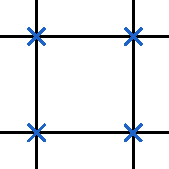
\includegraphics[width=.8\textwidth]{img/chapter4/the_method_grid_zoomed.pdf}};
                \draw[fill, color=ugent_blauw] (2.7,2) circle [radius=2pt] node[above right] {\Large ?};
            \end{tikzpicture}
        \end{center}
    \end{minipage}
    \hfill
    \begin{minipage}{.49\textwidth}
        \begin{center}
            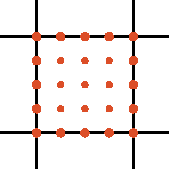
\includegraphics[width=.8\textwidth]{img/chapter4/the_method_grid_interpolate.pdf}
        \end{center}
    \end{minipage}
    \caption{On the left: a closer look at an internal rectangle from figure \ref{fig:woven_method_grid}. On the right: the points calculated with a small finite difference approximation.}\label{fig:c4_new_method_zoomed_in}
\end{figure}

But almost all points in the domain $\Omega$ are not contained on any of these lines. It is not trivial how one would now, from the results $\vb{c_x}$ and $\vb{c_y}$ from the matrix problem reconstruct the eigenfunction $\psi(x, y)$ in such a general point. Let us simplify the problem by only considering a rectangle between two consecutive grid lines, in both the x- and y-direction. The left side of figure \ref{fig:c4_new_method_zoomed_in} contains such a single rectangle. The question now is to reconstruct the eigenfunction on this rectangle, given its value on the whole boundary. Because we have to approximate an unknown function, given the values on a fixed number of points, interpolation comes to mind. As a first idea, we have tried building a polynomial basis to interpolate the eigenfunction with nodes on the boundary of such a rectangle.

\begin{figure}
    \begin{center}
        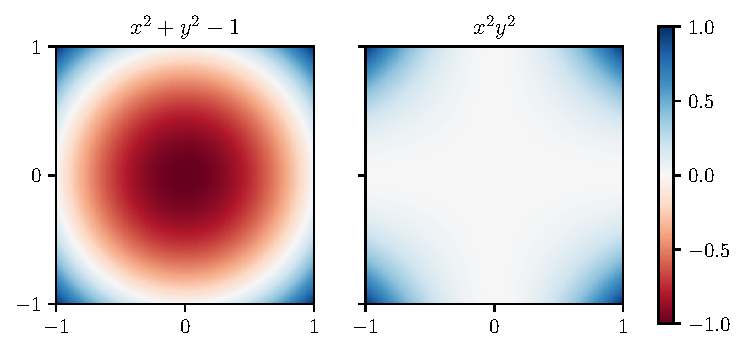
\includegraphics[width=1\textwidth]{img/chapter4/nm_interpolation.pdf}
    \end{center}
    \caption{Two different fourth degree polynomial functions with the same value on the boundary of the region $[-1, 1] \times [-1, 1]$.}\label{fig:c4_interpolation_boundary issue}
\end{figure}

The most natural $k$-degree polynomial basis to consider are for all $i, j$ the polynomials $x^i y^j$ with $i + j \leq k$. For $k = 4$, for example, this yields:
$$
    1\text{, } y\text{, } y^2\text{, } y^3\text{, } y^4\text{, } x\text{, } x y\text{, } x y^2\text{, } x y^3\text{, } x^2\text{, } x^2 y\text{, } x^2 y^2\text{, } x^3\text{, } x^3 y\text{ and } x^4\text{.}
$$
And this basis already highlights one of the fundamental issues with this approach. In figure \ref{fig:c4_interpolation_boundary issue} two different linear combinations of basis functions are plotted: $x^2 + y^2 -1$ and $x^2y^2$. Clearly, these functions are different. Yet, their value on the boundary of the unit square is identical. This indicates that it will not be possible to reconstruct the eigenfunction by using polynomial basis functions based upon only values from the boundary alone.

To be able to calculate an interpolating polynomial uniquely we also require values in the interior of the domain. The vectors $\vb{c_x}$ or $\vb{c_y}$ provide the value of the eigenfunction on the boundary of the small internal rectangle. They tell us nothing about the value of the eigenfuntion in the interior. But, on this internal rectangle $\Omega_{i, j} = [x_i, x_{i+1}] \times [y_j, y_{j+1}]$ we know that the eigenfunction $\psi(x, y)$ satisfies the Schrödinger-like equation
\begin{equation}\label{equ:c4_interpolation_schrodinger}
    -\nabla^2 \psi(x, y) + V(x, y) \psi(x, y) = E \psi(x, y)
\end{equation}
with $E$ fixed and boundary conditions:
\begin{align*}
    \psi(x_i, y)                 & = \sum_{k=0}^\infty c_k^{(x_i)} \beta_k^{(x_i)}(y)\text{,}          \\
    \psi(x_{i+1}, y)             & = \sum_{k=0}^\infty c_k^{(x_{i+1})} \beta_k^{(x_{i+1})}(y)\text{,}  \\
    \psi(x, y_j)                 & = \sum_{k=0}^\infty c_k^{(y_j)} \beta_k^{(y_j)}(x)                  \\
    \text{and } \psi(x, y_{j+1}) & = \sum_{k=0}^\infty c_k^{(y_{j+1})} \beta_k^{(y_{j+1})}(x) \text{.}
\end{align*}

Using this, we place a $K \times K$ grid on this small rectangular domain $\Omega_{i, j}$, as in the right-hand side of figure \ref{fig:c4_new_method_zoomed_in}. The grid points can now be described as $x_i = x^{(i)}_0$, $x^{(i)}_1$, $\dots$, $x^{(i)}_m$, $\dots$, $x^{(i)}_K = x_{i+1}$, and analogous for $y$: $y_j = y^{(j)}_0$, $y^{(j)}_1$, $\dots$, $y^{(j)}_n$, $\dots$, $y^{(j)}_K = y_{j+1}$. This allows the eigenfunction $\psi(x, y)$ to be approximated in each of these points by:
$$
    \psi^{(i,j)}_{m,n} \approx \psi(x^{(i)}_m, y^{(j)}_n) \quad \text{ for each $m, n \in \{0, 1, \dots, K\}$.}
$$
With this notation in hand, equation \ref{equ:c4_interpolation_schrodinger} can be approximated in each grid point by a finite difference approximation. Because $\Omega_{i,j}$ is only a small part of the total domain $\Omega$, the grid size $K$ may be chosen relatively small, without a penalty on accuracy. In our case, we found that fixing $K = 4$ gives satisfactory results, without too much computational overhead. So for the following discussion about a finite difference approximation on $\Omega_{i,j}$, we assume $K = 4$.

Because only a relatively small grid is used, the finite difference scheme should be as accurate as possible, without making any assumptions on points outside $\Omega_{i,j}$. Denote with $f''_0$ the value we want to approximate on an equidistant grid on which the function in question takes the values $\dots, f_{-2}, f_{-1}, f_{0}, f_{1}, f_{2}, \dots$ around the central point. The finite difference approximation can be written as
$$
    f''_0 \approx \sum_{i = a}^{b} \alpha_i f_i
$$
with appropriate choices for $a$ and $b$ such each $f_i$ lies within the grid of approximations. The relevant five-point formula we will be using are provided in the following table.

\begin{center}
    \begin{tabular}{@{}ccc|c|ccc@{}}
        $-3$                               & $-2$            & $-1$            & $0$            & $1$             & $2$             & $3$             \\ \hline
        \rule{0pt}{3ex}                    &                 & $\frac{11}{12}$ & $\frac{-5}{3}$ & $\frac{1}{2}$   & $\frac{1}{3}$   & $\frac{-1}{12}$ \\
        \rule{0pt}{3ex}                    & $\frac{-1}{12}$ & $\frac{4}{3}$   & $\frac{-5}{2}$ & $\frac{4}{3}$   & $\frac{-1}{12}$ &                 \\
        \rule{0pt}{3ex}    $\frac{-1}{12}$ & $\frac{1}{3}$   & $\frac{1}{2}$   & $\frac{-5}{3}$ & $\frac{11}{12}$ &                 &
    \end{tabular}
\end{center}

Let us, for ease of notation, summarize these values into the following matrix:
$$
    \vb{D} = \begin{pmatrix}
        0                             & 0            & 0            & 0            & 0             \\
        \rule{0pt}{3ex} \frac{11}{12} & \frac{-5}{3} & \frac{1}{2}  & \frac{1}{3}  & \frac{-1}{12} \\
        \rule{0pt}{3ex} \frac{-1}{12} & \frac{4}{3}  & \frac{-5}{2} & \frac{4}{3}  & \frac{-1}{12} \\
        \rule{0pt}{3ex} \frac{-1}{12} & \frac{1}{3}  & \frac{1}{2}  & \frac{-5}{3} & \frac{11}{12} \\
        0                             & 0            & 0            & 0            & 0
    \end{pmatrix}\text{.}
$$
With this finite difference approximation \eqref{equ:c4_interpolation_schrodinger} can now be approximated as a nine-dimensional linear system: for each $m, n \in \{1,2,3\}$:
$$
    \begin{cases}
        \qquad\vdots                                                                                                                                                                                                 \\
        {\displaystyle \sum_{l=0}^4 \frac{D_{m, l}}{\Delta x_i^2}\psi^{(i,j)}_{l, n} + \sum_{l=0}^4 \frac{D_{n, l}}{\Delta y_j^2}\psi^{(i,j)}_{m, l} =  \left(V(x^{(i)}_m, y^{(j)}_n) - E\right)\psi^{(i,j)}_{m, n}} \\
        \qquad\vdots
    \end{cases}
$$
The nine unknown variables are $\psi^{(i, j)}_{m, n}$ for $m, n \in \{1,2,3\}$. The step sizes $\Delta x_i$ and $\Delta x_j$ are defined as $\left(x_{i+1} - x_{i}\right) / K$ and $\left(y_{i+1} - y_{i}\right) / K$ respectively. Notice that for all $m, n \in \{0,1,\dots, K\}$, if any of $m, n \in \{0, 4\}$ the values $\psi^{(i, j)}_{m, n}$ are known, as they can be computed as the boundary values.

This relatively small linear system can now be numerically solved to obtain values of the eigenfunction within the small rectangle $\Omega_{i,j}$. On the right-hand side of figure \ref{fig:c4_new_method_zoomed_in}, all red dots are now computed values and can be used to construct a polynomial interpolation. As a basis we have chosen the 25 functions: $x^i y^j$ for all $i,j \in \{0,1,2,3,4\}$.


\subsubsection{Alternative methods}

Throughout the development of an algorithm to compute values of the eigenfunctions, we have considered many other methods for the computation of these eigenfunctions on an interior rectangle as well. In this section we will acknowledge some of these alternatives, together with their strengths and weaknesses. To motivate our final idea of solving a tiny Schrodinger-like problem to find interior points to interpolate through, a modest numerical comparison will be studied.

\paragraph{Interpolation through only boundary points} Previously, we stated that the functions $x^2 + y^2 - 1$ and $x^2 y^2$ have an identical boundary on the square $[-1, 1] \times [-1, 1]$. Also recall figure \ref{fig:c4_interpolation_boundary issue}. This non-uniqueness can be solved by only considering polynomials with a total degree strictly less than four:
$$
    1, x, y, x^2, xy, y^2, x^3, x^2 y, x y^2 \text{ and } y^3\text{.}
$$
These ten functions can now be used as an interpolation basis. For this we choose ten points on the boundary of the internal rectangle. Or, we choose more points and use a least squares approximation.

\todo{Interpolation up to cubic functions}

\todo{Interpolation over different small rectangles}

\todo{$K > 4$, trade off between runtime and accuracy}

\subsubsection{Non-rectangular domains}

\todo{Non-rectangular domains}

\subsection{Numerical experiments}\label{sec:c4_numerical_experiments}

When developing a new method it is instrumental these are well tested. This inescapably means that the program should be run on many problems with a wide variety of settings. Doing this thoroughly and consistently after code changes can be a cumbersome task. Knowing this, we have from the very first versions onwards included many automatic tests. On every code change, these tests would run on all supported platforms (Linux, Windows and macOS) to verify that our changes still produce sufficiently accurate results for the considered problems. For the development of this new method we continuously test the harmonic oscillator, the Hénon-Heiles potential and the quartic oscillator (\ref{sec:c4_numerical_harmonic} and \ref{sec:c4_numerical_henon_heiles}) on simple rectangular domains, the zero potential (\ref{sec:c4_numerical_zero}) on a rectangular and circular domain and Ixaru's potential on a rectangular, circular and a $45\degree$ rotated rectangle. All tests are conducted in \texttt{double}-precision and most problems are also tested in de extended \texttt{long double} datatype.

These automated tests are extremely valuable during development to quickly notice regressions. But for a thorough mathematical analysis more work is required. In this section we will provide many graphs and figures to evaluate the accuracy of our method. The evaluation of the runtime performance is another can of worms which will be treated in section \ref{sec:c4_nm_runtime}.

\subsubsection{Harmonic oscillator}\label{sec:c4_numerical_harmonic}

Following section \ref{sec:c4_fd_numerical}, the first example we will consider is the harmonic oscillator with equation
\begin{equation}\label{equ:c4_nm_harmonic}
    -\nabla^2 \psi(x, y) + \left(x^2 + y^2\right) \psi(x, y) = E \psi(x, y)
\end{equation}
on the domain $[\numprint{-9.5}, \numprint{9.5}] \times [\numprint{-9.5}, \numprint{9.5}]$ with homogeneous Dirichlet boundary conditions.

\begin{figure}
    \begin{center}
        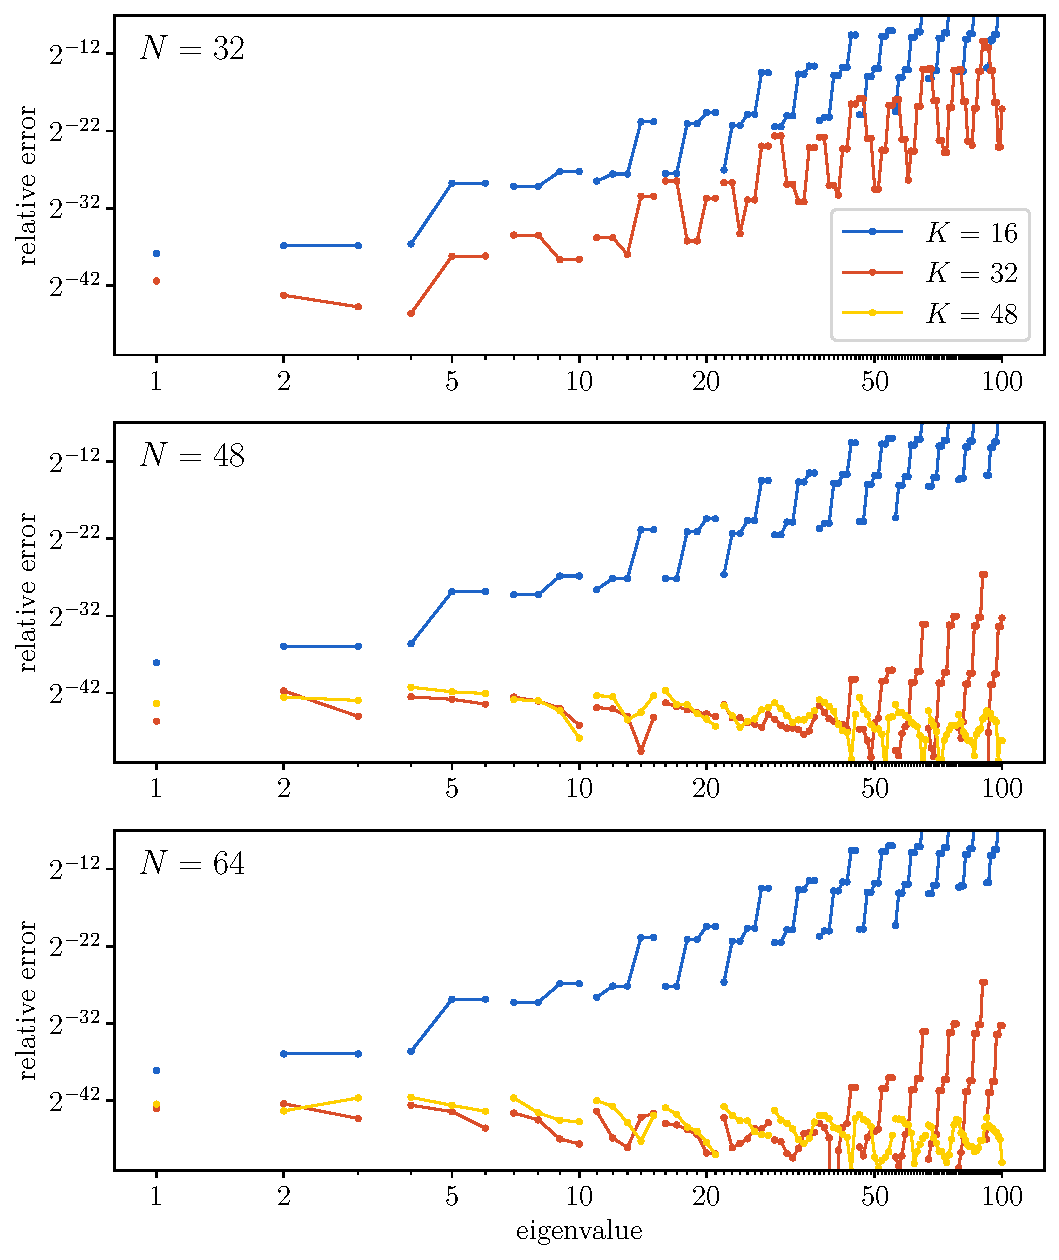
\includegraphics[width=\textwidth]{img/chapter4/nm_test_harmonic.pdf}
    \end{center}
    \caption{These graphs display the relative error of each of the first $100$ eigenvalues of the harmonic oscillator \eqref{equ:c4_nm_harmonic} on a rectangular domain $[-9.5,9.5]\times[-9.5, 9.5]$, computed for different grid sizes $N$ and basis sizes $K$. Repeated eigenvalues are connected.}
    \label{fig:c4_nm_harmonic_rectangle}
\end{figure}

In our algorithm there are two main variables to experiment with. The first, most obvious one, is the density of the used grid. This density lies in line with the grid approximation of the method that uses a finite difference approximation. In our method the size of the involved matrices, and thus the runtime, is directly proportional to the total number of grid points. Being able to use a less dense grid would therefor bring a significant computational benefit to the table.

The second parameter we can tweak is the number of basis functions on each of the grid lines. On each grid line, in both directions, \matslise needs to compute these basis functions. This computation requires, of course, a part of the runtime. In a very crude analysis we can take a look at the computational complexity of both operations. Assume there are $N$ grid lines in both directions. This yields $N^2$ grid points, and $2N$ grid lines. On each of these lines we compute $K \leq N$ basis functions, thus the computational overhead of the many one-dimensional problems is $\OO(K N)$. For the computation of the eigenvalues of the two-dimensional problem, the analysis is more nuanced. Finding accurate and reliable complexity estimates is a more difficult than one would expect. The restarted Arnoldi procedure (without shift-Invert), has a complexity of $\OO(k^2 n)$ when $k$ eigenvalues are requested for a sufficiently sparse $n \times n$ matrix\cite{lee_k2n_2009}. If the linear operator has a dense operation, this dominates the complexity $\OO(k n^2)$. In our case, we support a shift-invert scheme. In this scheme solving the sparse system is definitely something to take into account. \Eigen's built-in methods are based upon techniques from \superlu{}\cite{demmel_supernodal_1999,li_overview_2005}. In the performance analysis of this software, the authors provide a detailed overview of which properties have an impact on performance. An important property which contribute to the runtime is the structure of the matrix. If the non-zero elements of the involved matrix are so situated that the algorithm can exploit it, it helps the computational cost. It is not known whether our matrix has an exploitable structure or not. It would be surprising if our matrix had the perfect structure, independent of the size and shape of the domain.

In summary, a first complexity analysis of our method indicates that the one-dimensional problems have a complexity of $\OO(K N)$ and solving the matrix eigenvalue problem has a complexity of at least $\OO(k N^2)$. One has to be wary to only rely on a theoretical analysis to conclude that solving the one-dimensional problems has a negligible computational cost. In section \ref{sec:c4_nm_runtime} we will conduct a thorough analysis of the runtime of our method. For now, we will focus on numerical accuracy.

Figure \ref{fig:c4_nm_harmonic_rectangle} contains three graphs illustrating how the two main variables (grid size and basis size) work together to obtain accurate results. For this figure three different basis sizes were considered $K = 16$, $K = 32$ and $K = 48$. As grid sizes we have chosen $N = 32$, $N = 48$ and $N=64$. Notice that $N = 32$ and $K = 48$ was omitted from the figure as these give exactly the same results as $N = 32$ and $K = 32$, due to the limitation that the number of basis functions can never exceed the number of grid points on the relevant grid line.

Upon close inspection of the comparison of figure \ref{fig:c4_nm_harmonic_rectangle} with figure \ref{fig:c4_fd_harmonic}, we notice that our new method is able to reach the same accuracy with only a grid size of $48$ (with $48$ basis functions). This is considerably less than the required grid size of $100$ with spacing $h = 0.19$ when using the finite difference scheme.

\begin{figure}
    \begin{center}
        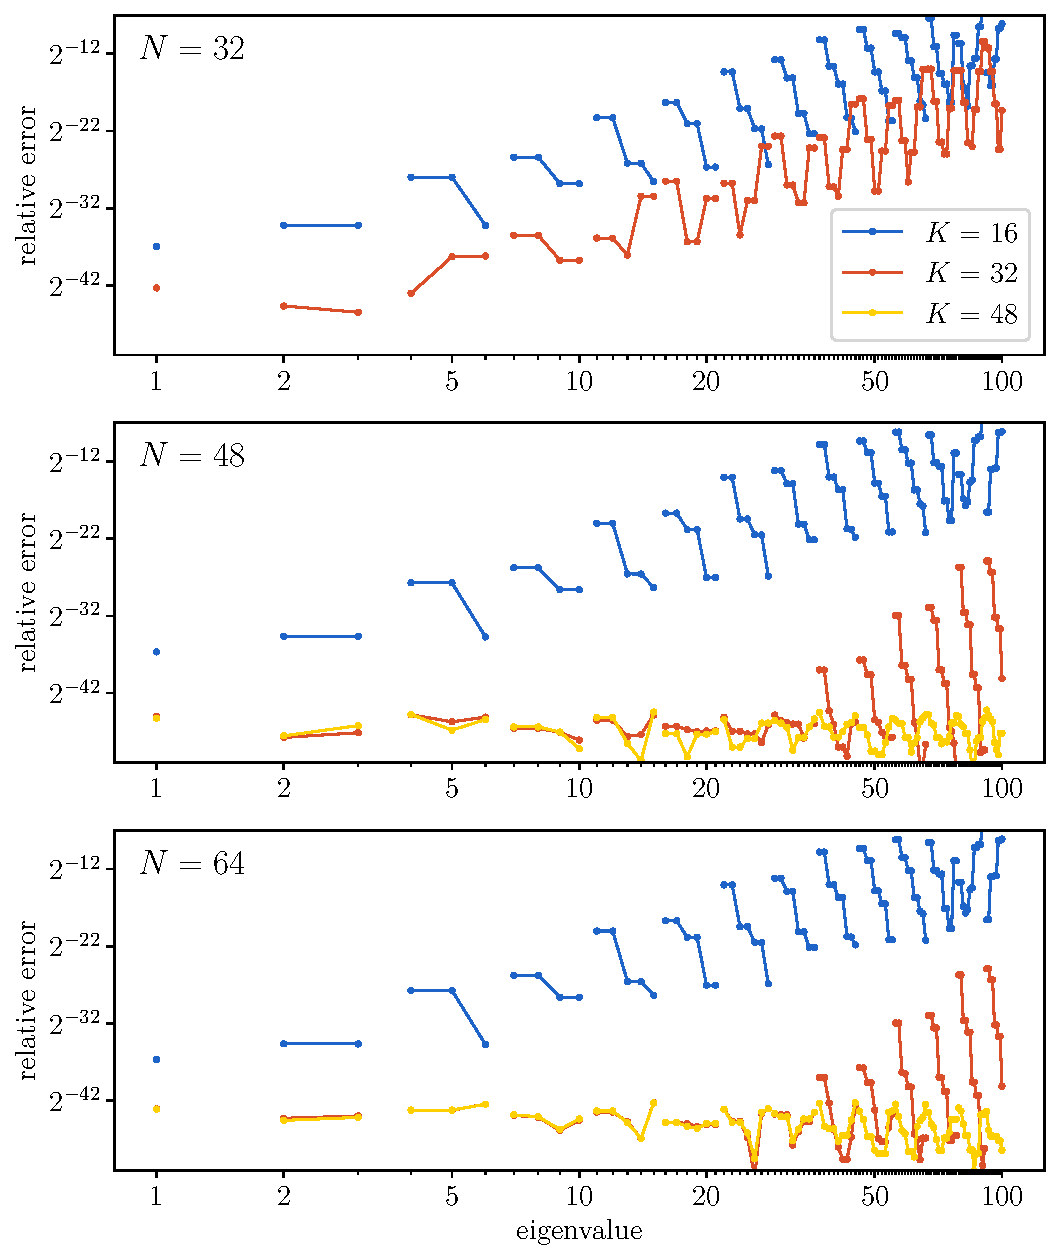
\includegraphics[width=\textwidth]{img/chapter4/nm_test_harmonic_disc.pdf}
    \end{center}
    \caption{These graphs display the relative error of each of the first $100$ eigenvalues of the harmonic oscillator \eqref{equ:c4_nm_harmonic} on the disc around $\vb{0}$ with radius $9.5$, computed for different grid sizes $N$ and maximal basis sizes $K \leq N$. On every line, the used basis size will be limited to the number of grid points on that line. Repeated eigenvalues are connected.}
    \label{fig:c4_nm_harmonic_disc}
\end{figure}

As a second, highly related experiment we try the harmonic oscillator, equation \eqref{equ:c4_nm_harmonic} on a circular domain around $(0, 0)$ with radius $9.5$. In principle, this is the same problem as before. But in practice, solving Schrödinger problems on non-rectangular domains was not at all possible with other grid-based methods.

Because we have constructed this method with non-rectangular domains in mind, ours is able to tackle these more exotic problems. Figure \ref{fig:c4_nm_harmonic_disc} answers for this problem the most important question: are the results accurate? The graphs displayed in this figure are calculated in the same way as figure \ref{fig:c4_nm_harmonic_rectangle}. Three different grid sizes and three different maximal basis sizes are considered. Notice that we used the term \emph{maximal} basis size. For non-rectangular domains the number of grid points per grid line varies. Grid lines close to the boundary are short chords containing only a few grid points. As the number of points limits the size of the basis, the true basis size has to vary as well. For our algorithm it is still valuable to place an upper bound on the basis size, especially for those lines that run through the middle of the domain, with many containing grid points.

\begin{figure}
    \begin{center}
        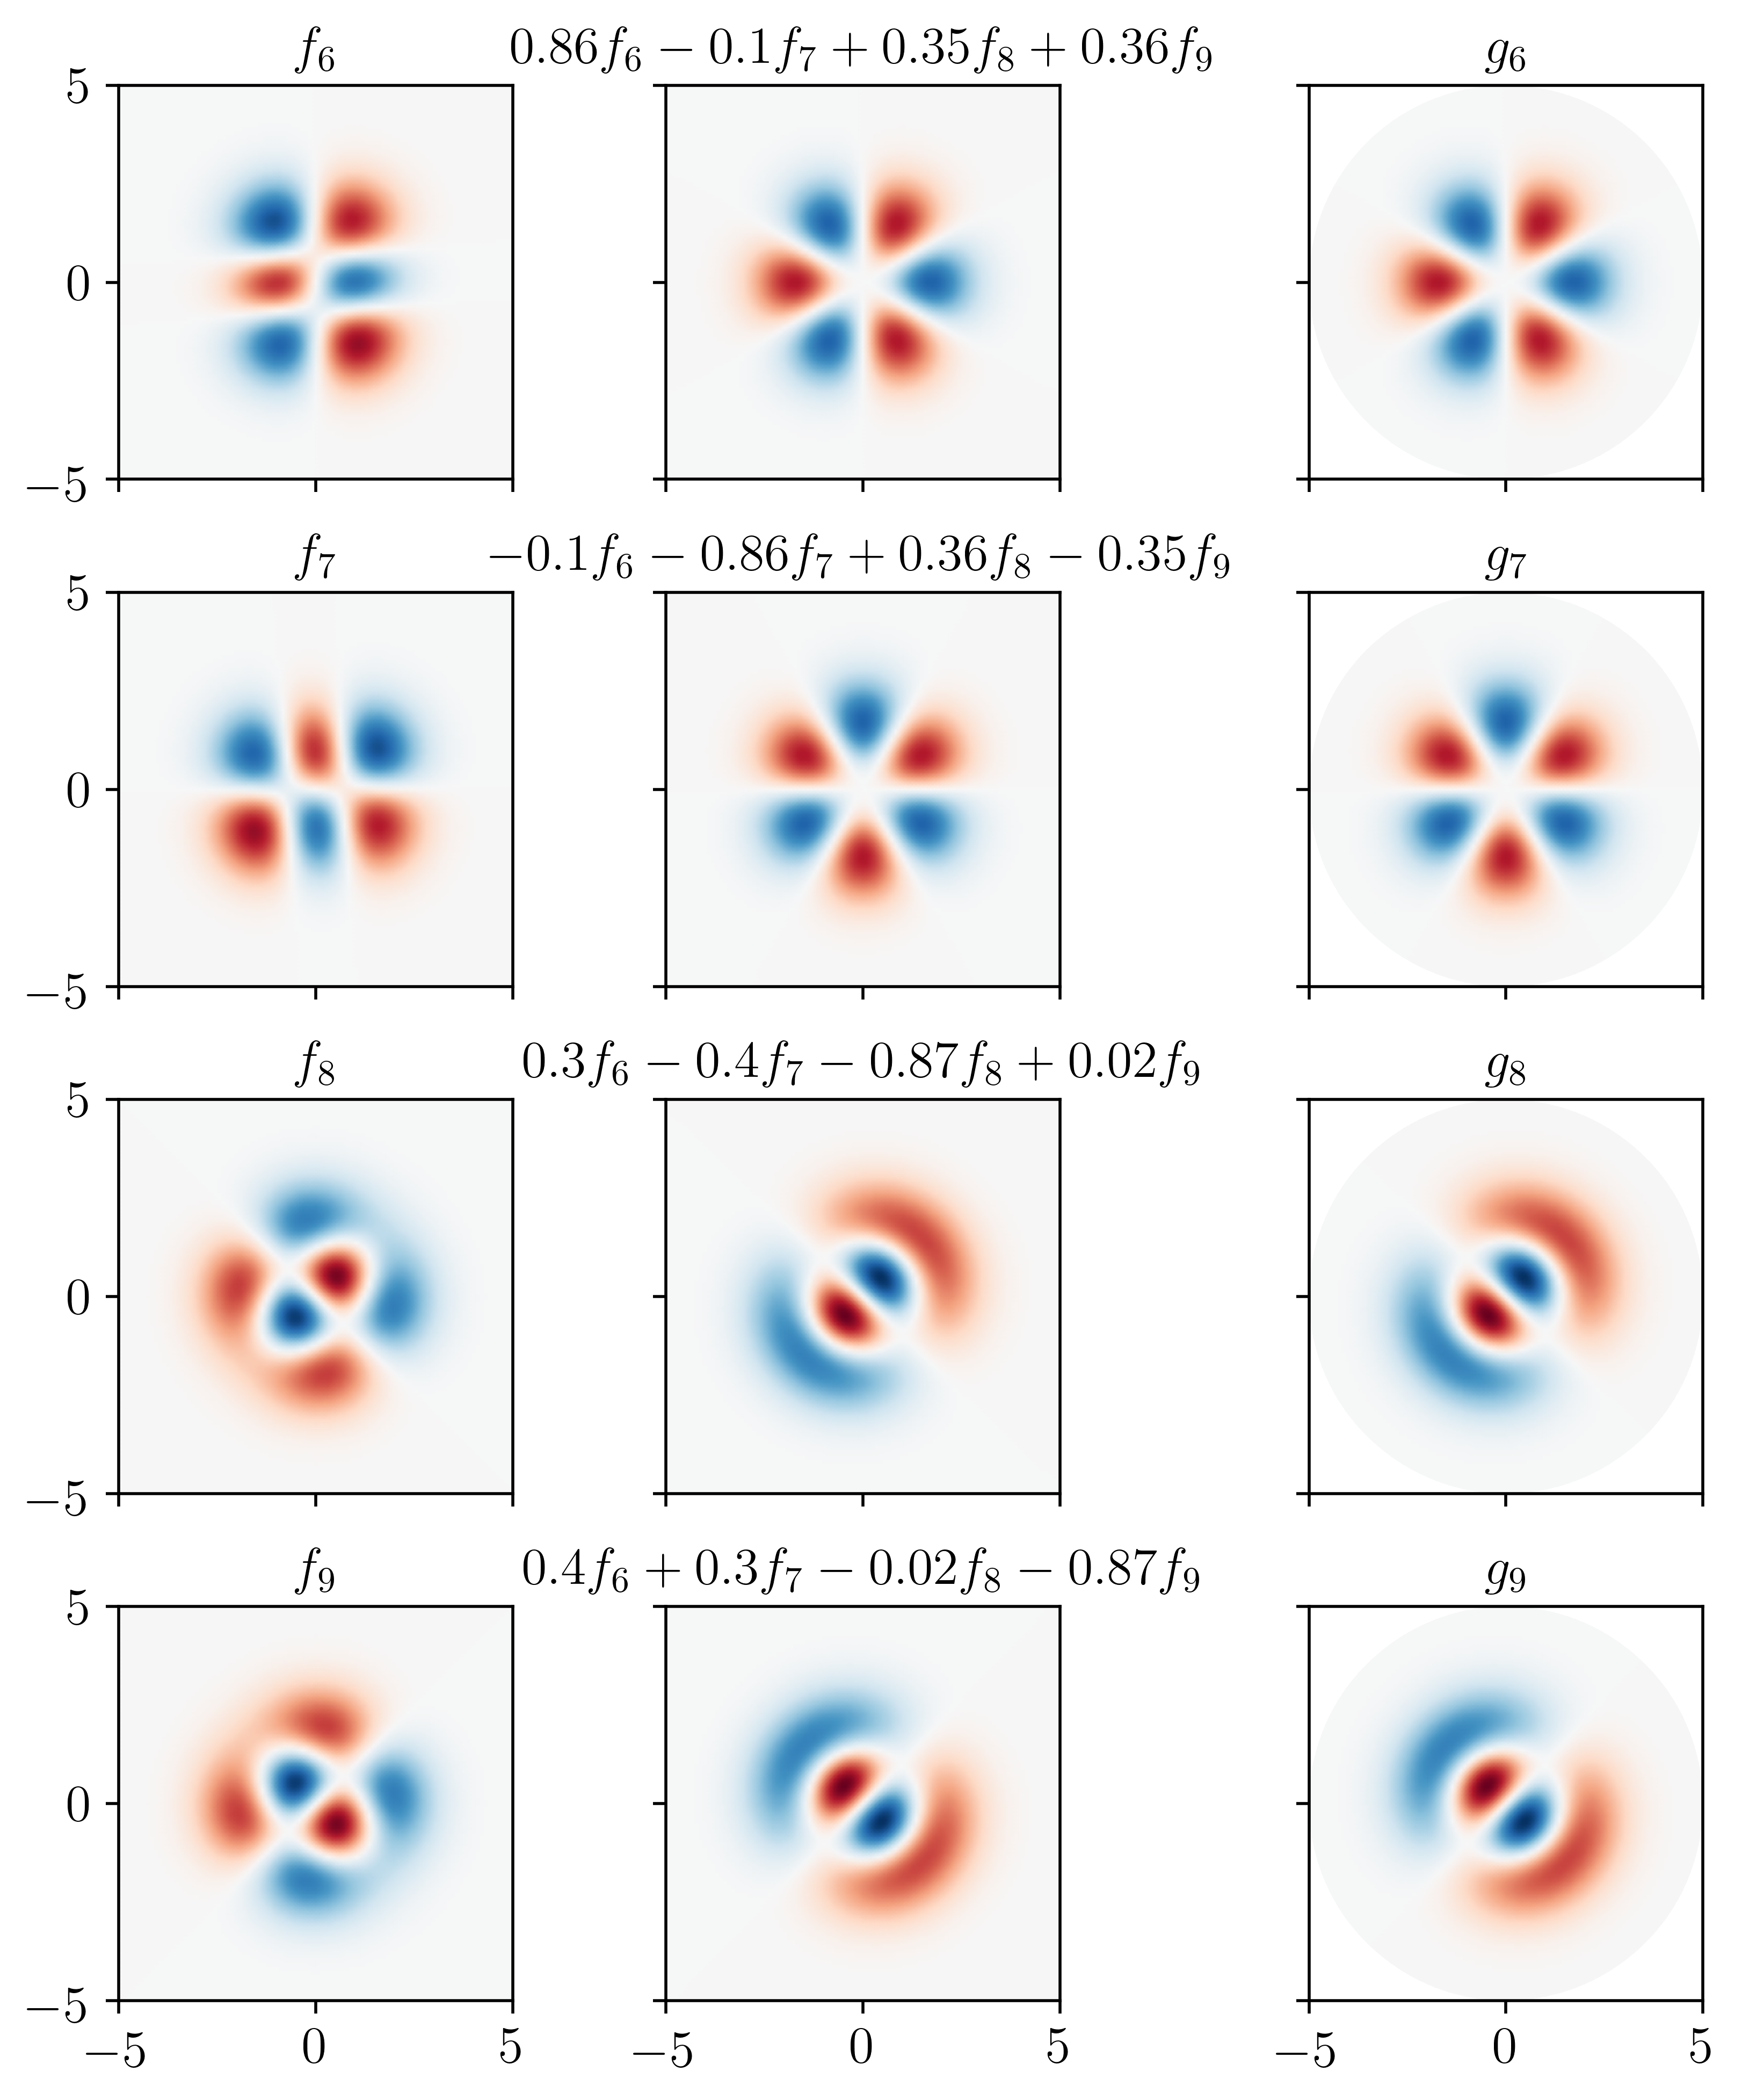
\includegraphics[width=\textwidth]{img/chapter4/nm_test_harmonic_eigenfunctions.png}
    \end{center}
    \caption{Left: four eigenfunctions with the same eigenvalue of the harmonic oscillator on the rectangular domain $[-5, 5]$. Right: the corresponding eigenfunctions on the circular domain with radius $5$. Middle: linear combinations of the left eigenfunctions are chosen such that they equal the right eigenfunctions.}
    \label{fig:c4_nm_harmonic_eigenfunctions}
\end{figure}

The results of figure \ref{fig:c4_nm_harmonic_disc} are eerily similar to those of figure \ref{fig:c4_nm_harmonic_rectangle}. For the harmonic oscillator the domain seems to have no effect on the accuracy of the method. This can be explained by the fact that for all eigenfunctions $f(\vb{x})$: $\lim_{\|\vb{x}\| \to +\infty} f(\vb{x}) = 0$. As a consequence this means that once the domain is sufficiently large the boundary, and corresponding boundary conditions, become less and less important. One of the great benefits of considering this circular domain is its size. For example, if $N = 64$ the rectangular domain has $4096$ grid points. The circular domain on the other hand, only has $3300$ grid points. This reduction in grid points makes the involved matrices smaller, and therefor reduces the computational cost.

As a last visual experiment with the harmonic oscillator, we will take a look at the eigenfunctions. As a reminder: the true eigenfunctions of the two-dimensional harmonic oscillator are:
$$
    2, 4, 4, 6, 6, 6, 8, 8, 8, 8, 10, 10, 10, 10, 10, 12, \dots
$$
Figure \ref{fig:c4_nm_harmonic_eigenfunctions} plots a basis for all eigenfunctions corresponding to eigenvalue $\lambda_6 = \lambda_7 = \lambda_8 = \lambda_9 = 8$. In the left-most column the basis for the eigenfunctions on the square domain $[-5, 5] \times [-5, 5]$ can be seen, and in the right-most column the basis found on a circular domain around zero with radius $5$. We have opted here for a smaller domain, not because of computational cost, on the larger domain these eigenfunctions can be drawn just as quickly. But, because of visual usefulness. On a larger domain, the interesting center part of the image would be a lot smaller and thus less visible.

Upon a first viewing of these eigenfunctions (left and right columns) one may be surprised that these are different. But, as the eigenspace corresponding to eigenvalue $8$ is multidimensional the basis is no longer unique. To be able to compare these results we have introduced the middle column. Here, a linear combination of basis functions from the rectangular domain is calculated such that we obtain the same basis functions as found on the circular domain. This illustrates some of the challenges when trying to compare or numerically verify eigenfunctions.

\subsubsection{Zero potential}\label{sec:c4_numerical_zero}

Analogous to section \ref{sec:c4_fd_numerical}, the next example we will study is the zero potential. Here the Schrödinger equation simplifies to:
$$
    -\nabla^2 \phi(x, y) = \lambda\phi(x, y)
$$
on the domain $\Omega$, with homogeneous Dirichlet boundary conditions.

If the domain $\Omega$ is the rectangle $[0, \pi] \times [0, \pi]$ exact solutions can be obtained with separation of variables. This gives $\forall i, j \in \Nplus$ that $i^2 + j^2$ is an eigenvalue of this Schrödinger problem with corresponding eigenfunction $\phi(x, y) = \sin(i x)\sin(j y)$.

\begin{figure}
    \begin{center}
        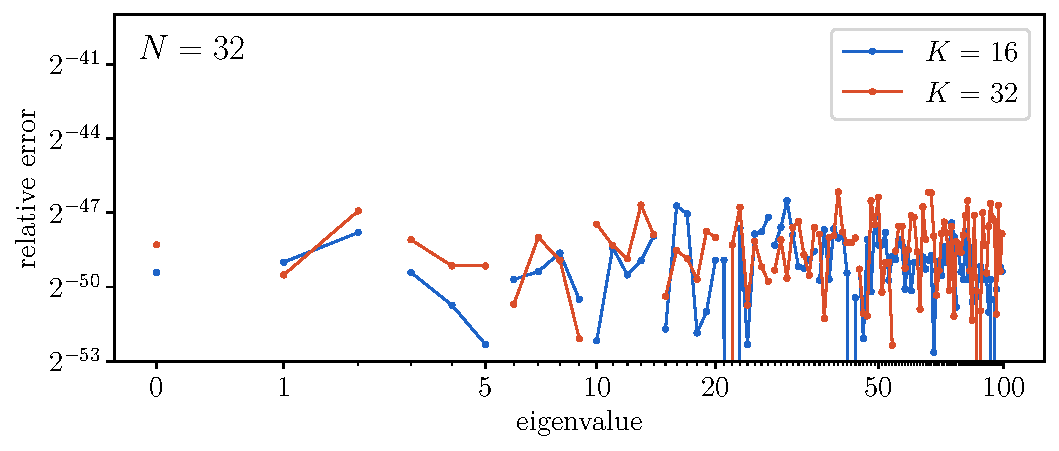
\includegraphics[width=\textwidth]{img/chapter4/nm_test_zero_rectangle.pdf}
    \end{center}
    \caption{This graph displays the results of our new method for the zero potential on the square $[0, \pi] \times [0, \pi]$, for a fixed grid size of $N = 32$ and a varying basis size. Notice the zoomed in y-axis, close to the machine precision of $2^{-53}$.}
    \label{fig:c4_nm_zero_test_rectangle}
\end{figure}

In figure \ref{fig:c4_nm_zero_test_rectangle} the results for this problem are visualized. Unsurprisingly, our method works extremely well for this. The main reason can be found in the fact that the basis functions \matslise calculates on each line are exactly $\sin(x)$, $\sin(2x)$, $\sin(3x)$\dots and analogous for $y$. These functions are able to exactly represent the true eigenfunctions $\sin(i x)\sin(j y)$ on each line.

\begin{figure}
    \begin{center}
        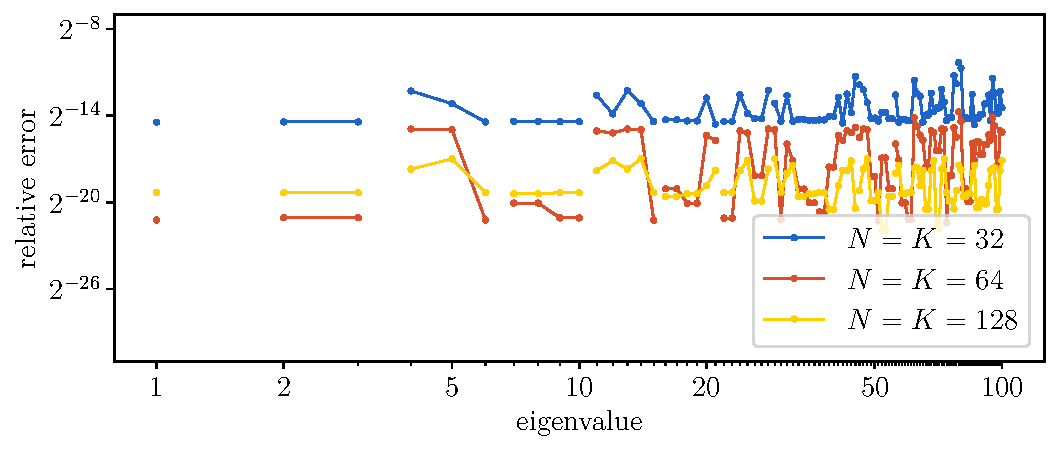
\includegraphics[width=\textwidth]{img/chapter4/nm_test_zero_disc.pdf}
    \end{center}
    \caption{This graph displays the results of our new method for the zero potential on the circular domain around $(0, 0)$ with radius $5$, for varying grid and basis sizes. Notice the shifted y-axis, to larger errors.}
    \label{fig:c4_nm_zero_test_disc}
\end{figure}

For non-rectangular domains with the zero potential, the story is different. Let us consider the Schrödinger equation with the zero potential and the circular domain around $(0, 0)$ with radius $1$ and homogeneous Dirichlet boundary conditions. The exact eigenvalues are known as the squares of the roots of the Bessel functions. See section \ref{sec:c3_eigenvalues_wrt_domain_analysis} for the full symbolic calculation.

The relative errors of the first hundred eigenvalues found with our new method are shown in figure \ref{fig:c4_nm_zero_test_disc}. We have tested this with the grid size and maximal basis size both equal to $32$, $64$ or $128$. The results are less impressive than for rectangular domains as the maximal accuracy reached is somewhere around $10^{-6}$. But nevertheless being able to compute these values at all is quite unique.


\subsubsection{Hénon-Heiles potential}\label{sec:c4_numerical_henon_heiles}

Another often used test problem is the Hénon-Heiles system. In the context of time-independent two-dimensional Schrödinger equations the potential in question is given as:
$$
    V(x, y) = x^2 + y^2 + \frac{3\sqrt{5}}{10}(3 x y^2 - x^3)\text{.}
$$
For a detailed analysis of this potential we refer back to section \ref{sec:c3_experiment_henon}.

\begin{figure}
    \begin{center}
        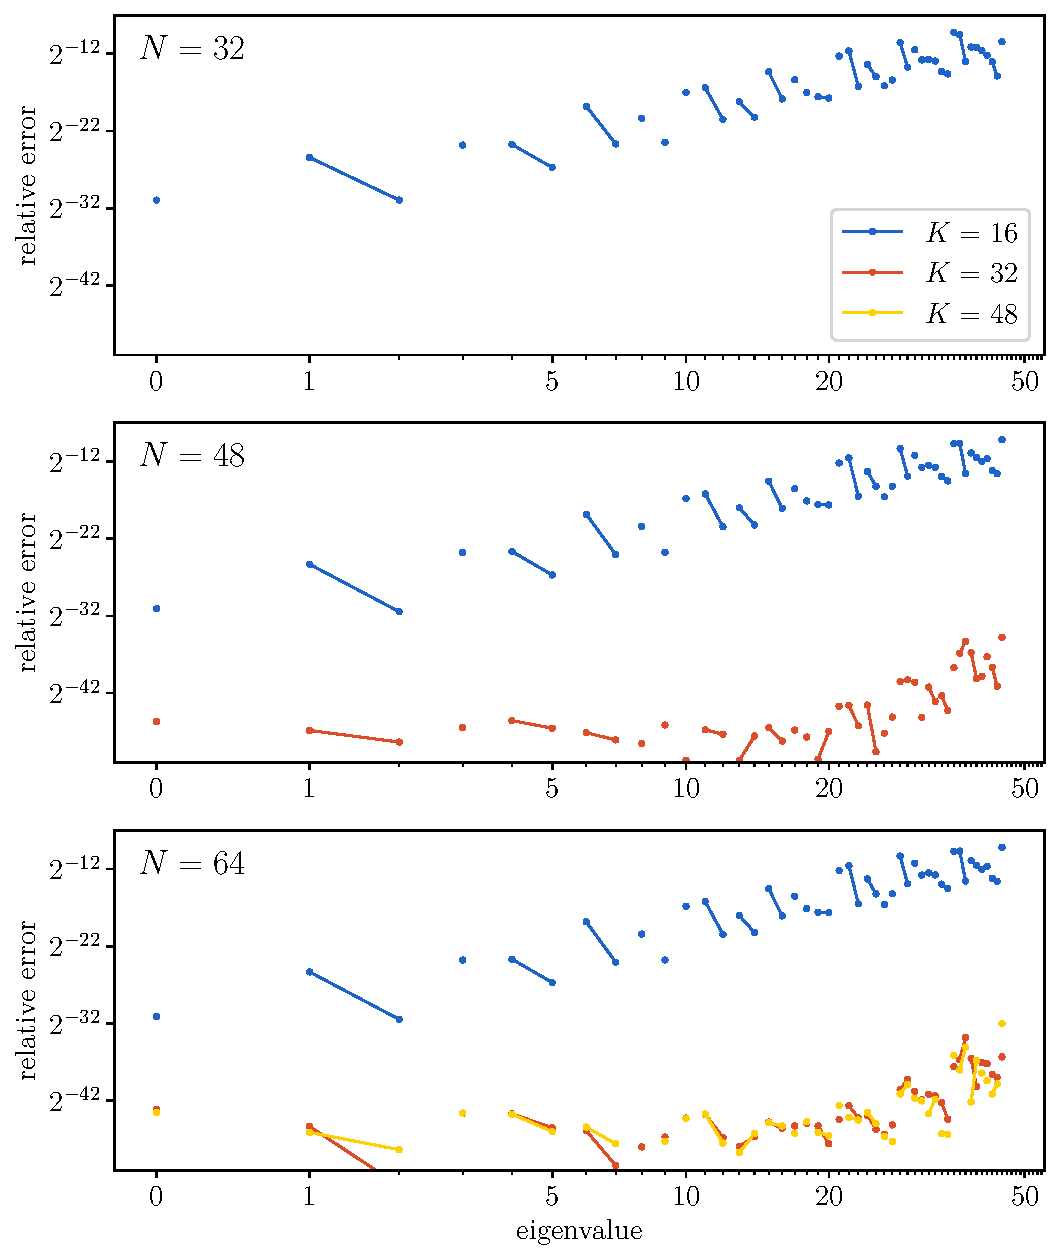
\includegraphics[width=\textwidth]{img/chapter4/nm_test_henon.pdf}
    \end{center}
    \caption{These graphs display the relative errors when we compare the results from our method with those from \cite{wang_new_2009} for the Hénon-Heiles system on the domain $[-10, 10]\times[-10, 10]$. For the parameters $N = K = 32$ and $N = K = 48$, our method found some physically nonsensical eigenvalues and therefor are missing from the plots.}
    \label{fig:c4_nm_henon_test}
\end{figure}

In \cite{wang_new_2009}, the authors remark to take care when choosing the size of the domain. This should not be too small to allow the eigenfunctions to converge to zero on the boundary. But it should neither be too large, because this can generate some physically nonsensical eigenvalues. They take as domain $[-10, 10] \times [-10, 10]$ and leave it at that. Looking at the available literature about this problem we find for example \cite{davis_semiclassical_1979}. Here, the proposed method does not use a clear defined boundary, but uses infinite basis functions. But, the interesting regions of these basis functions are only present in a radius, much smaller than $10$, around zero. \cite{braun_efficient_1996} limits their grid to a $[-6, 6] \times [-6, 6]$ domain. And in \cite{baeyens_improvements_2022}, the authors follow \cite{braun_efficient_1996}. For this experiment we will also take a $[-10, 10] \times [-10, 10]$ domain.

In figure \ref{fig:c4_nm_henon_test} the relative errors obtained with our method our displayed for this experiment. We used the results from \cite{wang_new_2009} as reference. Before analyzing these results we need to mention that for $N = K = 32$ and $N = K = 48$ our method found many nonsensical small eigenvalues. We know that they have no physical meaning because the corresponding eigenfunctions are only non-zero inside the valleys at the boundary. These unwanted eigenvalues disappear if the domain would be a little smaller, such that it no longer contains any valleys at the boundary.

Ignoring these special cases allows us to interpret the graphs from figure \ref{fig:c4_nm_henon_test}. Even on a small grid $N = 48$ we are able to accurately determine the eigenvalues. We also see that for the high eigenvalues increasing the grid size or basis size seems to have no effect. This is unexpected and seems to indicate that maybe the reference values are not perfect. The relative error for these high eigenvalues is $< 2^{-32} \approx 10^{-10}$ which is nonetheless extremely accurate.

\subsubsection{Ixaru's potential}\label{sec:c4_numerical_ixaru}

\todo{Ixaru's}

\subsection{Runtime analysis}\label{sec:c4_nm_runtime}

Throughout the development of this new method we have focussed upon keeping the matrices small. The idea is that finding eigenvalues of a (sparse) matrix is quite expensive, definitely more expensive than all other steps. But it would be careless to take this assumption at face value without more thorough analysis. In section \ref{sec:c4_numerical_experiments} we have already seen that our method can reach the same accuracy as a finite difference scheme with a smaller sparse matrix in the end. So, if all steps to construct the sparse problem are almost negligible in comparison to finding eigenvalues of that sparse system, then our method will be faster for the same accuracies.

As a first experiment, we will take a look at the Hénon-Heiles problem from section \ref{sec:c4_numerical_henon_heiles} on the square domain $[-6 , 6]\times [-6, 6]$ on a $64\times 64$ grid and a maximum basis size of $48$. We have run a profiler on our program to solve this problem. Our program consists of two main parts. First, the grid is constructed and the basis functions on each grid line are computed. Secondly, we employ \spectra to find the eigenvalues of the resulting sparse matrix. For the second part, we have two options. We can find the largest eigenvalues of the shifted inverse matrix. Or, with the implicitly started Arnoldi method we can select only the smallest eigenvalues while converging. The first technique has much better convergence, but is more expensive because in each step a linear system has to be solved. For many problems the second technique also converges to the true smallest eigenvalues, but the convergence is less reliable and slower. But the final runtime may be faster because no systems have to be solved.

To evaluate these differences we have solved this problem 20 times with each of the techniques (selecting the smallest eigenvalues versus using the shifted inverse matrix). With the first technique, our program had an average total runtime of $\numprint[s]{3.295}$ and with the second technique the total runtime rose to $\numprint[s]{8.700}$. Using only these numbers to draw conclusions may be a little premature.

In both cases, the construction of the grid and the determining of the basis functions are identical. In the following table we have summarized the averaged results from the profiler. All reported times are the average of 20 runs, with no deviation of more than $5\%$ between runs.

\begin{center}
    \begin{tabular}{lrr}
	 & calls & runtime \\
	\hspace{0mm}construct grid and solve one-dimensional problems & $1$ & $\numprint[ms]{531}$ \\
	\hspace{5mm}finding a basis on a single grid line & $128$ & $\numprint[ms]{436}$ \\
	\hspace{5mm}evaluate each eigenfunction in all grid points & $6144$ & $\numprint[ms]{89}$\end{tabular}{lrr}
    
\end{center}

The `calls' column contains the total number of times that function was executed, the `runtime' column contains the total time that was spent inside this function. So the construction of the grid took $\numprint[ms]{531}$ and was executed once (per run). On each grid line, the basis functions had to be found. Because we have chosen a $64 \times 64$ grid, this function was called $128 = 64 + 64$ times. In this function our program constructs a \matslise object to find the first $48$ eigenvalues, for each of these eigenvalues the eigenfunction is also calculated, but not yet evaluated. The evaluation of these functions is done a few moments later when constructing the relevant $\vb{B_x}$ and $\vb{B_y}$ matrices. A total of $\numprint{6144} = 48 \cdot 128$ eigenfunctions were evaluated with a total runtime of $\numprint[ms]{89}$. The other steps within this construction (such as determining the boundaries of the domain, allocating matrices or keeping track of grid points) only took on average $\numprint[ms]{6}$. So this table contains the most expensive functions in the construction of the problem.

To compute the eigenvalues themselves, we will first study the technique of the implicitly restarted Arnoldi iteration with selection of the lowest $100$ eigenvalues. For this Hénon-Heiles problem the correct results are found. But, we expect that the convergence may be slow. The following table contains the profiler's summary.
\begin{center}
    \begin{tabular}{l|r|r}
	 & calls & runtime \\
\hline	\hspace{0mm}computing eigenvalues & $\numprint{1}$ & $\numprint[ms]{2772}$ \\
	\hspace{5mm}SPECTRA compute eigenvalues & $\numprint{1}$ & $\numprint[ms]{2656}$ \\
	\hspace{10mm}perform operation & $\numprint{1316}$ & $\numprint[ms]{1151}$
\end{tabular}

\end{center}
We see that the computation for this part took \numprint[s]{2.772}. Together with the construction, this gives the total runtime of $\numprint[s]{3.295}$. We also see that SPECTRA called our matrix-free operation procedure \numprint{1316} times. The computation of this procedure took less than half the total time, the other time is spent inside the implicitly restarted Arnoldi iteration algorithm of \spectra.

Comparing this to the following table where the summary of the profiler is displayed when the eigenvalue algorithm is applied to the shifted inverse matrix.
\begin{center}
\begin{tabular}{lrr}
	 & calls & runtime \\
	\hspace{0mm}computing eigenvalues (shiftInvert) & $1$ & $\numprint[ms]{8289}$ \\
	\hspace{5mm}sparse LU-decomposition & $1$ & $\numprint[ms]{3731}$ \\
	\hspace{5mm}SPECTRA compute eigenvalues & $1$ & $\numprint[ms]{4529}$ \\
	\hspace{10mm}perform operation & $353$ & $\numprint[ms]{4166}$\end{tabular}{lrr}

\end{center}
Here we see that the convergence is faster, it is to say fewer operations are needed. But the runtime \numprint[s]{8.289} is much higher. The cause is twofold. First we see that before calling the eigenvalue routine we have to compute the sparse LU-decomposition of the involved matrix. This alone takes more time than the computation without inverse matrix. But even though almost four times fewer operations are needed to reach convergence, each operation is almost 14 times slower. This negates all benefits of the `faster' convergence.

The main take-away from these tables is that the construction time is dwarfed by the time effectively converging to the requested eigenvalues, regardless of the used method. But only looking at fixed parameters may be misleading. In figure \ref{fig:c4_benchmark_timings} we have plotted the true runtime of the construction time and the computation of the eigenvalues (with both techniques) for different parameters $N \in \{32,48,64,80,96,112\}$ and $K = \frac{3}{4}N$.

\begin{figure}
    \begin{center}
        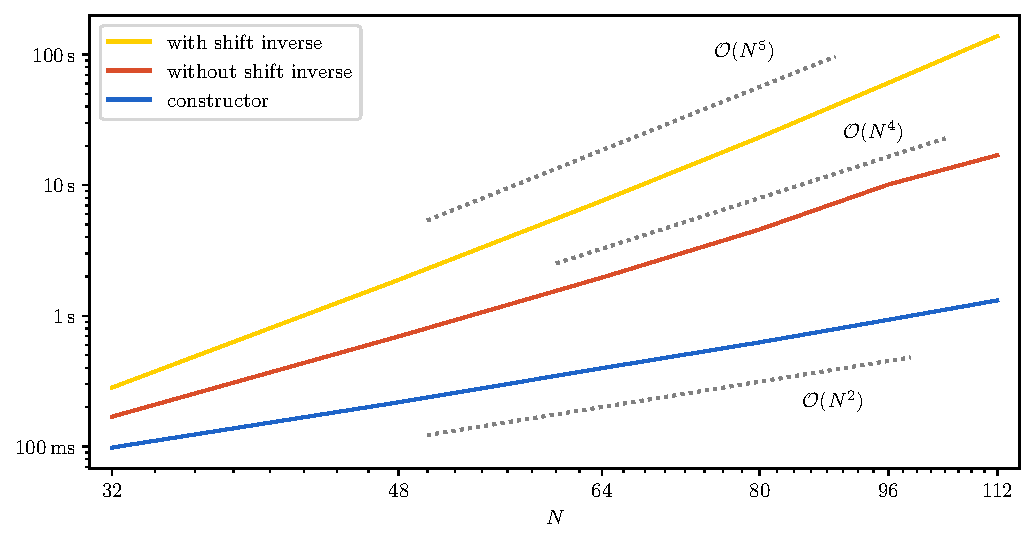
\includegraphics[width=\textwidth]{img/chapter4/benchmark/benchmark_timings.pdf}
    \end{center}
    \caption{The Hénon-Heiles problem on a $[-6,6] \times [-6,6]$ square domain is solved for parameters $N \in \{32,48,64,80,96,112\}$ and $K = \frac{3}{4}N$. The average runtime (over five runs) of the construction of the grid (with solving all one-dimensional subproblems) and of the computation of the eigenvalues with and without inverting the matrix are reported.\label{fig:c4_benchmark_timings}}
\end{figure}

In this figure we see that the construction of the grid (with solving all one-dimensional problems) has an experimental time complexity of $\OO(N^2)$. This is in line with our expectation. We have $2 N$ one-dimensional problems to solve, and for each of these problems $\frac{3}{4}N$ eigenvalues are requested. Now, in principle we have a $\OO(N^3)$ runtime complexity, because we will evaluate each of the $\frac{3}{2} N^2$ eigenfunctions in $N$ points. But, as seen from the detailed profiler results from before, this evaluation is quite efficient and as such this theoretic cubic complexity will not be present in practice. 

When we are using the shifted inverse matrix to find eigenvalues, we can see an experimental runtime of $\OO(N^5)$. A dense LU-decomposition has a cubic complexity in the size of the involved matrix. In our case a sparse LU-decomposition is calculated of the $N^2 \times N^2$ sparse matrix. This decomposition is able to exploit some sparsity and as such we hope (and expect) a speed-up. This is what we see with the measured $\OO(N^5)$ complexity.

When the eigenvalues are found by selecting the smallest values during convergence a theoretical analysis is more difficult. In a single step our matrix-free operation computes deflated vectors and a matrix-vector product. The former is computed with sparse basis vectors, the latter is computed with a sparse matrix. Let us focus on the main matrix-vector product. This matrix is given in the right-hand side of equation \eqref{equ:c4_nm_sparse_system}. The first term is a block diagonal-matrix with $N$ $K\times K$-blocks. The second term has a similar but permuted structure. Therefor, each row contains at most $2K - 1$ non-zero entries, for a total of $\OO(N K^2) = \OO(N^3)$ non-zero entries. The bases of the deflation spaces are similarly sparse. For determining the total time complexity, `only' an estimate for the number of operations is needed. But, in most analyses of this eigenvalue solver it is assumed that the outer boundary of the spectrum is selected in each step, not the smallest values. So finding reliable estimates is quite difficult. Using the experiment from figure \ref{fig:c4_benchmark_timings} we can suspect that the number of steps before convergence is $\OO(N)$, which is the square root of the matrix size.

But in any case, our focus on reducing the matrix-size has been worthwhile. The main bottleneck is still the computation of the eigenvalues for which many well-tested extremely-efficient and even parallelly distributed algorithms exist. In comparison to \cite{wang_new_2009}, our method is able to reach the same or higher accuracies (as discussed in section \ref{sec:c4_numerical_experiments}) with smaller grid sizes, and thus matrix sizes, which in turn reduces the total runtime.

\subsection{The name Strands}

When developing and publishing a new method maybe one of the most difficult challenges (besides developing, testing, analyzing, implementing\dots the method) is probably finding a fitting name. As mathematicians, we may sometimes forget the importance of a recognizable name. But let's take a look at some names we encounter in the area of Schrödinger equations. For the one-dimensional method we have for example SLEDGE, SLEIGN, SLCPM12 and Matslise itself. For the system of coupled equations we have LILIX or Matscs. For the specific two-dimensional problem we have not found any packages with memorable names. But if we look a bit further to the libraries we used: Eigen (\cpp library for linear algebra), Spectra (\cpp library for finding eigenvalues), PETSc and SLEPc (scalable c-libraries for linear algebra). We also came across Numpy and SciPy as numerical libraries in Python. Or, we can look at the wider scientific computing community for inspiration: BLAS and LAPACK (interfaces for basic linear algebra), Armadillo (\cpp library for linear algebra), GNU GSL (scientific computing in C), SageMath (a computer algebra system), Maple (program for symbolic computation), FEniCS with DOLPHIN (platform to solve partial differential equations), OpenFOAM (for computational fluid dynamics),

A name should be short and be more or less relevant to the method. The names I like the most are the pronounceable fun names (with bonus points if it is a backronym\footnote{Wikipedia tells us: ``a backronym is an acronym formed from an already existing word". For example: Spectra stands for ``\emph{Sp}arse \emph{E}igenvalue \emph{C}omputation \emph{T}oolkit as a \emph{R}edesigned \emph{A}RPACK.}) like LILIX, Spectra, Sage and FEniCS.

When first developing the ideas for this method I always saw it as a loom, with warp and weft threads. The tension ensures that in the grid points these threads intersect. There are many fun words in the weaving-industry for which a backronym could be found, but these are always quite niche and not well-known. But after a short conversation with ChatGPT it proposed `Stranded Schrödinger Solver' as name. And I liked the word \emph{strand} a lot. It is synonymous with \emph{thread} and \emph{wire}, so it fits definitely with my mental model of the method. But, \emph{strand} is also the Dutch word for \emph{beach}, which brings the `fun' aspect back to the table. And as our method uses many strands together, this gives us:

% Logo idea: two pair orthogonaly intersecting harmonic eigenfunctions

\begin{center}
    \begin{minipage}{.8\textwidth}
        \begin{description}
            \item[\textbf{Strands}] \hfill\\ \textbf{St}anding waves app\textbf{r}oxim\textbf{a}tions for the $\bm{n}$-\textbf{d}imensional \textbf{S}chrödinger problem (with $n = 2$ and maybe in the future $n = 3$).
        \end{description}
    \end{minipage}
\end{center}

\section{Some ideas for a utopian method}\label{c4:sec_utopy}

In the introduction of this chapter we briefly discussed what a perfect method for time independent Schrödinger equations may be. It should be a method which is fast and accurate, of course. More specifically, its accuracy should not degrade upon requesting higher eigenvalues. Even if ridiculously high eigenvalues are required. But, ideally, this guaranteed accuracy should not come with the cost of increased run time. Requesting the first five eigenvalues should be (approximately) as fast as requesting the five eigenvalues larger than one million for example.

In this section, I want to give an overview of the ideas and experiments I explored in the past few years. This section will not be written as a scientific paper. It will not contain absolute truths. It will not allege to have any certainties. This section will contain many of my mathematical feelings, unverified, uncensored, and definitely not peer reviewed. And, I will try highlight in which ideas I still see merit, and with which ideas I have run into a dead end.

Before diving into my mathematical ramblings, I need to give you some caveats: I have not read every article about the topics described here. I do not know all intricacies of developing numerical methods. And I see myself as an applied mathematician\footnote{This is not an apology, I am a proud (and proudly) applied mathematician. But, my background influences how I practice mathematics. And in this section in particular this is important to keep in mind when following along with my thoughts.}, so I prefer numerical experiments and testing a hypothesis over strong mathematical rigor and watertight proofs. Still, I believe myself to be somewhat qualified to write about numerical methods for two-dimensional time independent Schrödinger equations, as I spent the previous (almost) six years of my professional time developing such methods myself. But, if you have invested yourself in any of the topics we will cover here, and you find me to be unjustly negative or unfairly harsh, I really do want to apologize in advance for that. It is not my intention to write theories off. It is not my intention to declare topics a waste of time. All things I write here are and will be my experience with these topics, in and only in the context of numerical methods for the two-dimensional time independent Schrödinger equation.

\subsection{Preliminary ideas}

\subsubsection{Exponential fitting}

The first topic I want to cover here is already controversial. My research group and in particular my promotor are already studying exponential fitting for over three decades. They were able to successfully use this technique countless times in various applications. And, I know, as a young researcher, even younger than they have been researching this topic even, it is quite pretentious to make statements about this topic. But my promotor and I have worked sufficiently close together, that he knows me to make some statement I better should not have. Let this subsection be such a statement.

The general idea of exponential fitting is to develop methods which are specifically tuned to be accurate for exponential and oscillatory function of certain frequencies. They have been successfully applied to numerical differentiation, quadrature formulas and ordinary differential equations (linear multistep methods and Runge-Kutta methods)\cite{ixaru_exponential_2004}. For the more recent advances we refer to \cite{paternoster_present_2012}. The success of this technique can not be denied.

Yet, my relationship with exponential fitting has been rocky. Most importantly, this thesis could not have come to fruition without them. The constant perturbation methods, and in particular \matslise, are exponentially fitted methods. The extreme accuracies reached for the one-dimensional problem are only possible because for each energy the specifically tuned $\eta$-functions take exactly the important frequencies into account.

On the other hand, when we tried to use exponentially fitted quadrature formulas for the computation of the potential matrix $\vb{V}^{(k)}(y)$ in section \ref{sec:c3_calculate_vk}, the results were less than ideal. It was already quite the challenge to determine to which frequencies these formulae should be tuned. Because these quadrature formulae should be computed for many possible eigenvalues and for all sectors of the domain with a wildly varying potential, the fitted frequencies most definitely could not be constant. So they should be automatically and dynamically computed. In principle this only incurs a small computational overhead. In practice, this was quite difficult to implement. We needed to tune the formulae for different frequencies and many edge-cases arose: what if some of them were close together? What if some functions were exponential and the others trigonometric? Or all exponential? Or none of them? All these question were interconnected, and important. If two frequencies were close together, in the formulae we were dividing two tiny numbers. So the limit had to be taken. In relatively rare cases the resulting quadrature formulae became highly unstable with large negative weights. One of the major issues was that even though these cases were quite rare, they popped up often because we were approximating so many integrals. In short, this instability caused a numerical mess. After this experience, I hope you can understand the hesitation in my love for exponential fitting.

The eigenfunctions of the two-dimensional eigenproblem we are trying to solve are oscillatory, even highly so for large eigenvalues. Therefor, it is natural to think about exponential fitting. But translating this idea into something practical is not straightforward. For ordinary differential systems much research from recent years is available: second order problems\cite{dambrosio_exponentially_2011,}, symplectic methods \cite{vandenberghe_symplectic_2011,wu_explicit_2012}\dots For partial differential equations we have found very little research available. In \cite{zahra_exponentially_2019} the authors develop an exponentially fitted method for the two-dimensional time fractional damped Klein-Gordon equation. Upon construction of the symbolic formulae they use a polynomial basis set together with the following exponential functions, based upon the parameters $\mu, \nu \in \CC$:
$$
    \exp(\pm\mu x \pm\nu y), x\exp(\pm\mu x \pm\nu y), y\exp(\pm\mu x \pm\nu y), x y \exp(\pm\mu x \pm\nu y), \dots
$$
For determining $\mu$ and $\nu$ they propose an algorithm which is able to eliminate the leading term of the error by choosing these parameters appropriately. In our case, using this set of basis functions directly will be far from optimal. For the Schrödinger equation, we have seen that the frequency of the oscillations is highly dependent on the value of the potential. Where in the domain the potential is low, the eigenfunction will strongly oscillate, where the potential is higher the oscillations will slow down, and where the potential is even higher than the energy there will be no oscillations at all, and we have an exponential behavior. So in a certain sense, the values of $\mu$ and $\nu$ should dependent upon the energy and upon the value of the potential, and by extension thus the location $x, y$ in the domain.


\subsubsection{Piecewise constant approximations}

\todo{Canosa and De Oliveira first ideas, high level overview and quick sketch for 2D}

\subsubsection{Constant perturbation}

\todo{Without being negative: why it is secondary to the constant approximation}

\subsubsection{Shooting}

\todo{Shooting vs direct methods, why we need shooting for high eigenvalues}

\subsubsection{Finding eigenvalues within an order of magnitude}

\todo{Like Prüfer}

\subsection{The main idea}

\todo{Some formulas, boundary conditions, propagation, CP?}



\stopchapter
